\documentclass[11pt,a4paper]{article}

\usepackage[margin=2.4cm]{geometry}
\usepackage[utf8]{inputenc}
\usepackage{lmodern}
\usepackage[T1]{fontenc}
\usepackage{amsmath,amssymb,amsfonts,amsthm}
\usepackage{mathtools}
\usepackage{booktabs}
\usepackage{array}
\usepackage{enumitem}
\usepackage{graphicx}
\usepackage{listings}
\usepackage{xcolor}
\usepackage{hyperref}
\hypersetup{colorlinks=true, linkcolor=blue, citecolor=blue, urlcolor=blue}

\lstset{
  language=Python,
  basicstyle=\ttfamily\footnotesize,
  keywordstyle=\bfseries,
  commentstyle=\itshape\color{gray},
  breaklines=true,
  frame=single,
  columns=fullflexible,
  keepspaces=true,
  showstringspaces=false,
  aboveskip=0.6em,
  belowskip=0.6em,
}

\theoremstyle{plain}
\newtheorem{theorem}{Teorema}
\newtheorem{lemma}[theorem]{Lema}
\newtheorem{proposition}[theorem]{Proposici\'on}
\newtheorem{corollary}[theorem]{Corolario}

\theoremstyle{definition}
\newtheorem{definition}{Definici\'on}
\newtheorem{remark}{Observaci\'on}
\newtheorem{assumption}{Hip\'otesis}

\newcommand{\vect}[1]{\boldsymbol{#1}}
\newcommand{\matr}[1]{\mathbf{#1}}
\newcommand{\R}{\mathbb{R}}
\newcommand{\N}{\mathbb{N}}
\newcommand{\softplus}{\operatorname{softplus}}
\newcommand{\erf}{\operatorname{erf}}
\newcommand{\norm}[1]{\left\lVert #1 \right\rVert}
\newcommand{\abs}[1]{\left\lvert #1 \right\rvert}
\DeclareMathOperator{\diag}{diag}
\DeclareMathOperator{\Cov}{Cov}
\DeclareMathOperator{\sgn}{sgn}
\DeclareMathOperator{\supp}{supp}
\DeclareMathOperator*{\esssup}{ess\,sup}

\title{Un forward anal\'itico \emph{diferenciable} para el CRB de la
c\'amara de esquina activa\\[4pt]
\large De la \textbf{funci\'on del simulador} a derivadas cerradas (Camino A)}
\author{Obstacle Detection Study}
\date{\today}

\begin{document}
\maketitle

\begin{abstract}
Estas son \textbf{notas del ``por qu\'e''} de c\'omo volvimos
\emph{diferenciable} el forward que ya usa el simulador, para poder calcular el
Cram\'er--Rao (CRB) con \textbf{derivadas parciales cerradas} sin tocar el
simulador rasterizado (\texttt{pyerti.py},
\texttt{simulation\_polar\_clean.ipynb}, \texttt{crb\_polar\_functions.py}).
El punto de partida \textbf{no} es el modelo del \emph{writeup}, sino la
\emph{propia funci\'on del simulador}: el bucle de tri\'angulos de la celda~8 de
\texttt{simulation\_polar\_clean.ipynb} (l\'ineas $\sim$208--318), un modelo de
\textbf{dos rebotes} (l\'aser$\to$faceta$\to$p\'ixel de piso) cuya intensidad por
p\'ixel usa \textbf{cuatro cosenos} de \emph{foreshortening}, la constante
$4\pi^2$ y las dos distancias $d_1,d_2$. Identificamos sus \textbf{tres} fuentes
de no diferenciabilidad --- el binning temporal \texttt{ceil} (masa de Dirac en
un bin), el ocultamiento por umbral \texttt{xint}$>0$ (Heaviside) y los
\emph{clamps} \texttt{max}$(0,\cdot)$ en los cosenos --- y las reemplazamos, una
por una y justificando \emph{por qu\'e} cada elecci\'on, por an\'alogos suaves de
clase $C^\infty$: la masa de Dirac por la integral anal\'itica de un pulso
gaussiano (diferencia de $\erf$), el umbral por una sigmoide de penumbra, y los
\emph{clamps} por \emph{softplus}. Presentamos por separado, y ambas
\textbf{paso a paso}, una secci\'on de \textbf{construcci\'on} y otra de
\textbf{justificaci\'on matem\'atica}. Las derivadas se obtienen
\textbf{simb\'olicamente} con \texttt{sympy} (an\'alogo al Mathematica del
\emph{writeup}) y se validan contra diferencias finitas del mismo forward suave,
con error m\'aximo relativo $\sim\!1\times10^{-9}$. C\'odigo:
\texttt{crb\_analytic\_forward.py}; validaci\'on:
\texttt{validate\_analytic\_forward.py}. Importante: el CRB es funci\'on
\emph{solo del modelo} (no consume datos), y este forward anal\'itico es un
modelo \emph{aparte} --- no el simulador con sus salidas ``pasadas por funciones
suaves'' ---; la Sec.~\ref{sec:que-entra} aclara qu\'e entra al CRB y por qu\'e su
uso es leg\'itimo. Adem\'as, con \textbf{amplitud f\'isica} (\'area
$w\!\cdot\!h$ e \texttt{laser\_intensity} reales) y la \textbf{misma rejilla}
$64\times64$ y \texttt{bin\_size} del simulador, el CRB anal\'itico y el de la
ruta FD quedan en las \textbf{mismas unidades} / la misma escala f\'isica, a
diferencia de la versi\'on previa con ganancia y rejilla propias. \textbf{Ahora
bien}, esta variante \emph{no} converge a la FD: al ser una \textbf{cuadratura de
un solo punto} (radiometr\'ia en el centroide, \'area $w h$) mantiene un
\textbf{sesgo sistem\'atico} (sobreestima la intensidad $\sim1.5\times$, dominado
por la oclusi\'on de la faceta extendida) que \textbf{no desaparece} al endurecer
el suavizado --- al hacerlo converge a su \emph{propio} forward duro puntual, no
al de malla. La correcci\'on es la \textbf{suma sobre malla} (rama (a)+(b)+(c)).
\end{abstract}

\tableofcontents
\bigskip\hrule\bigskip

%==============================================================================
\section{El punto de partida: la funci\'on que usa el simulador}
\label{sec:partida}
%==============================================================================

El c\'alculo actual del CRB (documentado en \texttt{sustento\_teorico\_crb.tex})
diferencia por \textbf{diferencias finitas} el forward del simulador de
transporte de luz. Ese forward est\'a en el bucle de tri\'angulos de la celda~8
de \texttt{simulation\_polar\_clean.ipynb} (l\'ineas $\sim$208--318). Aqu\'i lo
transcribimos \emph{fielmente}, porque es \textbf{nuestro punto de partida}: la
funci\'on que queremos volver diferenciable, tal cual est\'a.

\paragraph{Geometr\'ia (dos rebotes).}
Para una pose $\vect{\psi}=(\rho,\varphi,h)$, la faceta ocupa $z\in[0,h]$; su
centroide (\emph{scene point}) --- el an\'alogo puntual del centro de masa de la
malla --- est\'a a media altura,
\begin{equation}
    \vect{p}_s=\bigl(\rho\cos\varphi,\ \rho\sin\varphi,\ \tfrac{h}{2}\bigr),
    \qquad
    \hat{\vect n}_s=(-\cos\varphi,\ -\sin\varphi,\ 0),
    \label{eq:pose}
\end{equation}
y el SPAD observa \emph{directamente} un punto de piso $\vect{p}_f$
(\texttt{cam\_pos}). \'Este es un modelo de \textbf{dos rebotes}
l\'aser$\to$faceta$\to$p\'ixel de piso (\textbf{no} tres): el l\'aser est\'a en
$\vect{p}_l=(0,0,0)$ con normal $\hat{\vect n}_l=(0,0,1)$, y el piso tiene normal
$\hat{\vect n}_f=(0,0,1)$. Se definen las dos distancias del camino
\begin{equation}
    \vect{lps}=\vect{p}_l-\vect{p}_s,\quad d_1=\norm{\vect{lps}};
    \qquad
    \vect{fovsp}=\vect{p}_f-\vect{p}_s,\quad d_2=\norm{\vect{fovsp}}.
    \label{eq:dist}
\end{equation}

\paragraph{Intensidad por p\'ixel (cuatro cosenos, $4\pi^2$).}
El simulador acumula la intensidad (celda~8, l\'ineas $\sim$283--308)
\begin{equation}
    \texttt{intensity}
    =
    I_{\mathrm{laser}}\; A\;
    \frac{\texttt{dot1}\cdot\texttt{dot2}\cdot\texttt{dot3}\cdot\texttt{dot4}}
         {4\pi^2\; d_1^2\; d_2^2},
    \label{eq:raster-int}
\end{equation}
con $A$ el \'area del tri\'angulo y los \textbf{cuatro cosenos} de
\emph{foreshortening}, cada uno con \emph{clamp} duro $[\,\cdot\,]_+=\max(0,\cdot)$:
\begin{equation}
\begin{aligned}
    \texttt{dot1}&=\Bigl[\hat{\vect n}_s\!\cdot\!\tfrac{\vect{p}_l-\vect{p}_s}{d_1}\Bigr]_+,
    &\quad
    \texttt{dot2}&=\Bigl[\hat{\vect n}_s\!\cdot\!\tfrac{\vect{p}_f-\vect{p}_s}{d_2}\Bigr]_+,\\[3pt]
    \texttt{dot3}&=\Bigl[\hat{\vect n}_l\!\cdot\!\tfrac{\vect{p}_s-\vect{p}_l}{d_1}\Bigr]_+,
    &\quad
    \texttt{dot4}&=\Bigl[\hat{\vect n}_f\!\cdot\!\tfrac{\vect{p}_s-\vect{p}_f}{d_2}\Bigr]_+ .
\end{aligned}
    \label{eq:raster-cos}
\end{equation}
(\texttt{dot1} y \texttt{dot3} son el \emph{foreshortening} en la faceta y en el
l\'aser sobre el tramo l\'aser$\to$faceta; \texttt{dot2} y \texttt{dot4}, en la
faceta y en el piso sobre el tramo faceta$\to$piso.)

\paragraph{Tiempo de vuelo y dep\'osito en bin.}
La intensidad se deposita \textbf{entera} en un \'unico bin entero de llegada
(l\'ineas $\sim$270--271):
\begin{equation}
    j \;=\; \left\lceil \frac{d_1+d_2}{c\,\Delta t} \right\rceil ,
    \label{eq:raster-ceil}
\end{equation}
i.e.\ una masa de Dirac en el tiempo de vuelo $t_0=(d_1+d_2)/c$.

\paragraph{Ocultamiento (m\'ascara dura).}
Solo se cuentan los p\'ixeles \emph{no ocluidos}. Con la recta faceta$\to$p\'ixel
en el plano $XY$ (l\'ineas $\sim$230--244),
\begin{equation}
    m=\frac{s_y-p_{f,y}}{s_x-p_{f,x}},\quad
    b_{\mathrm{line}}=s_y-m\,s_x,\quad
    \texttt{xint}=-\frac{b_{\mathrm{line}}}{m},\quad
    \texttt{noc}=\mathbf 1\{\texttt{xint}>0\},
    \label{eq:raster-noc}
\end{equation}
con $s_x=\rho\cos\varphi,\ s_y=\rho\sin\varphi$. Algebraicamente
\begin{equation}
    \texttt{xint}
    =
    s_x - s_y\,\frac{s_x-p_{f,x}}{s_y-p_{f,y}},
    \label{eq:xint}
\end{equation}
que es exactamente el \texttt{d\_edge} del c\'odigo actual.

\begin{remark}[Las tres operaciones que impiden $\partial g/\partial\vect{\psi}$ cerrada]
\label{rem:tres}
Todo lo dem\'as de \eqref{eq:raster-int}--\eqref{eq:xint} es \textbf{suave} en
$\vect{\psi}$: el \'area $A$, las distancias $d_1,d_2$, los productos internos
\emph{crudos} $\hat{\vect n}\!\cdot\!\vect u$, y la ca\'ida radial
$1/(4\pi^2 d_1^2 d_2^2)$. Las \textbf{tres} fuentes de no diferenciabilidad son,
exactamente:
\begin{enumerate}[nosep]
    \item \textbf{Binning \texttt{ceil}} \eqref{eq:raster-ceil}: masa de Dirac en
    un bin entero. $\lceil\cdot\rceil$ es constante a trozos; su derivada
    cl\'asica es $0$ salvo en saltos, donde no existe.
    \item \textbf{Ocultamiento} $\mathbf 1\{\texttt{xint}>0\}$
    \eqref{eq:raster-noc}: un Heaviside muestreado; derivada $=$ delta en la
    frontera iluminado/sombra.
    \item \textbf{\emph{Clamps}} $[\,\cdot\,]_+=\max(0,\cdot)$ en los cuatro
    cosenos \eqref{eq:raster-cos}: continuos pero con codo no derivable en $0$.
\end{enumerate}
Adem\'as el dep\'osito en \'indices enteros de p\'ixel/bin es intr\'insecamente
discreto. Por eso el pipeline vigente aproxima el Jacobiano por diferencias
finitas centrales y debe elegir con cuidado los pasos $\delta$. \emph{Volver
diferenciable} \eqref{eq:raster-int}--\eqref{eq:xint} es todo el problema.
\end{remark}

\begin{remark}[El \emph{writeup} solo como inspiraci\'on estructural]
\label{rem:writeup}
El modelo continuo del \emph{writeup} de la c\'amara de esquina activa (Seidel
\emph{et al.}) usa \textbf{tres} rebotes, \textbf{cinco} cosenos y un denominador
$8\pi^3$ (incluye la etapa c\'amara$\leftrightarrow$piso $\propto1/\norm{\vect
p_c-\vect p_f}^2$). \textbf{No} lo tomamos como base: nuestra construcci\'on parte
de la funci\'on del simulador \eqref{eq:raster-int} (dos rebotes, cuatro cosenos,
$4\pi^2$). Del \emph{writeup} reutilizamos \'unicamente (i) la \textbf{estructura
Poisson--Fisher} del CRB (Sec.~\ref{sec:fisher}) y (ii) la idea de \emph{derivar
bajo el integrando} con un sistema de \'algebra simb\'olica. Las elecciones de
suavizado (gaussiana$\to\erf$, sigmoide, softplus) se justifican por s\'i mismas
en la Sec.~\ref{sec:construccion}. La posici\'on de c\'amara $\vect{p}_c$ y la
distancia $\norm{\vect p_c-\vect p_f}$ \textbf{no} intervienen en el forward de
dos rebotes.
\end{remark}

%==============================================================================
\section{Construcci\'on de una versi\'on diferenciable (paso a paso)}
\label{sec:construccion}
%==============================================================================

Construimos un forward de \textbf{faceta puntual} que eval\'ua directamente el
integrando de \eqref{eq:raster-int} sobre una malla fija de p\'ixeles de piso
$\{\vect{p}_{f,i}\}$ y una rejilla fija de bins
$\{[t^{(j)}_{\mathrm{lo}},t^{(j)}_{\mathrm{hi}}]\}$, reemplazando cada operaci\'on
no diferenciable por su an\'alogo suave. Para cada una damos: \emph{c\'omo
estaba}, \emph{por qu\'e no es derivable}, \emph{con qu\'e se reemplaza} y
\emph{por qu\'e esa opci\'on}. El orden va de la pieza central hacia afuera.

%------------------------------------------------------------------------------
\subsection{(i) Binning temporal: de \texttt{ceil} a una diferencia de \texorpdfstring{$\erf$}{erf}}
\label{sec:erf}
%------------------------------------------------------------------------------

\textbf{C\'omo estaba.} La intensidad completa de un p\'ixel se deposita en un
\emph{\'unico} bin \eqref{eq:raster-ceil}: una masa de Dirac en
\begin{equation}
    t_0(\vect{\psi})=\frac{d_1(\vect\psi)+d_2(\vect\psi)}{c}
    =\frac{\norm{\vect{p}_s-\vect{p}_l}+\norm{\vect{p}_s-\vect{p}_f}}{c}.
    \label{eq:tof}
\end{equation}

\textbf{Por qu\'e no es derivable.} $\lceil\cdot\rceil$ es constante a trozos:
al mover $\vect{\psi}$, la masa \emph{salta} discretamente de un bin al vecino.
La derivada respecto de $\vect{\psi}$ es $0$ dentro de cada meseta y no existe en
el salto (v\'ease la Prop.~\ref{prop:fd}).

\textbf{Con qu\'e se reemplaza.} Por un \textbf{pulso gaussiano de \'area
unitaria} centrado en $t_0$,
\begin{equation}
    s(t)=\frac{1}{\tau\sqrt{2\pi}}\,
    \exp\!\left(-\frac{(t-t_0(\vect{\psi}))^2}{2\tau^2}\right),
    \qquad
    \int_{\R} s = 1,
    \label{eq:pulse}
\end{equation}
cuya integral sobre el bin $[t_{\mathrm{lo}},t_{\mathrm{hi}}]$ es \emph{cerrada}
(cambio $u=(t-t_0)/(\sqrt2\,\tau)$):
\begin{equation}
    \boxed{\;
    S_j(\vect{\psi})
    =\int_{t^{(j)}_{\mathrm{lo}}}^{t^{(j)}_{\mathrm{hi}}} s(t)\,dt
    =\frac{1}{2}
    \left[
        \erf\!\left(\frac{t^{(j)}_{\mathrm{hi}}-t_0(\vect{\psi})}{\sqrt2\,\tau}\right)
        -\erf\!\left(\frac{t^{(j)}_{\mathrm{lo}}-t_0(\vect{\psi})}{\sqrt2\,\tau}\right)
    \right].
    \;}
    \label{eq:erf-bin}
\end{equation}

\textbf{Por qu\'e esta opci\'on.} Tres razones: (1) el pulso f\'isico del
l\'aser/detector tiene \textbf{ancho temporal finito}, de modo que $\tau>0$ es
m\'as fiel que la idealizaci\'on Dirac, no un truco; (2) la gaussiana es
$C^\infty$ y su integral por bin es \textbf{cerrada} --- una diferencia de $\erf$,
funci\'on entera (Lema~\ref{lem:erf}) --- as\'i que $S_j$ es $C^\infty$ en
$\vect{\psi}$ a trav\'es de $t_0(\vect{\psi})$; (3) \textbf{conserva la masa}:
$\sum_j S_j\to1$, de modo que al sumar sobre bins se recupera la ``intensidad''
del rasterizador, pero ahora la masa se traspasa \emph{gradualmente} entre bins
vecinos. Esta es \textbf{la pieza central}. Por defecto
$\tau=\Delta t=3.9\times10^{-10}$\,s.

\paragraph{Convergencia, conservaci\'on de masa y el \emph{trade-off}.} El
parecido con la caja dura lo controla el cociente $\tau/\Delta t$: cuanto menor
es $\tau$, m\'as verticales son los flancos de $S_j$ y en el l\'imite
$\tau\to0^+$ se recupera exactamente el binning duro (consistencia,
Fig.~\ref{fig:smooth-binning}(a)). El criterio \emph{correcto} de validez, sin
embargo, no es el parecido visual sino la \textbf{conservaci\'on de masa}: para
\emph{todo} $\tau>0$ se cumple $\sum_j S_j(t_0)=1$ (la energ\'ia total del pulso se
reparte entre bins pero no se crea ni se destruye), como muestra la l\'inea plana
$\approx1$ de la Fig.~\ref{fig:smooth-binning}(b). Finalmente, la derivada
$\partial S_j/\partial t_0$ \eqref{eq:dS} es \textbf{continua y acotada} para
$\tau$ finito, pero \emph{se afila} (su pico crece $\sim1/\tau$ y se angosta)
conforme $\tau\to0$ (Fig.~\ref{fig:smooth-binning}(c)): \'ese es el \emph{trade-off}
suavidad$\leftrightarrow$fidelidad, y la raz\'on de que el l\'imite duro no sea
derivable (la derivada tiende a deltas). Mantener $\tau$ finito da lo mejor de
ambos: fidelidad razonable \emph{y} una derivada exacta y bien condicionada.

\begin{figure}[ht]
\centering
\IfFileExists{../plots/crb_smoothing_binning.png}{%
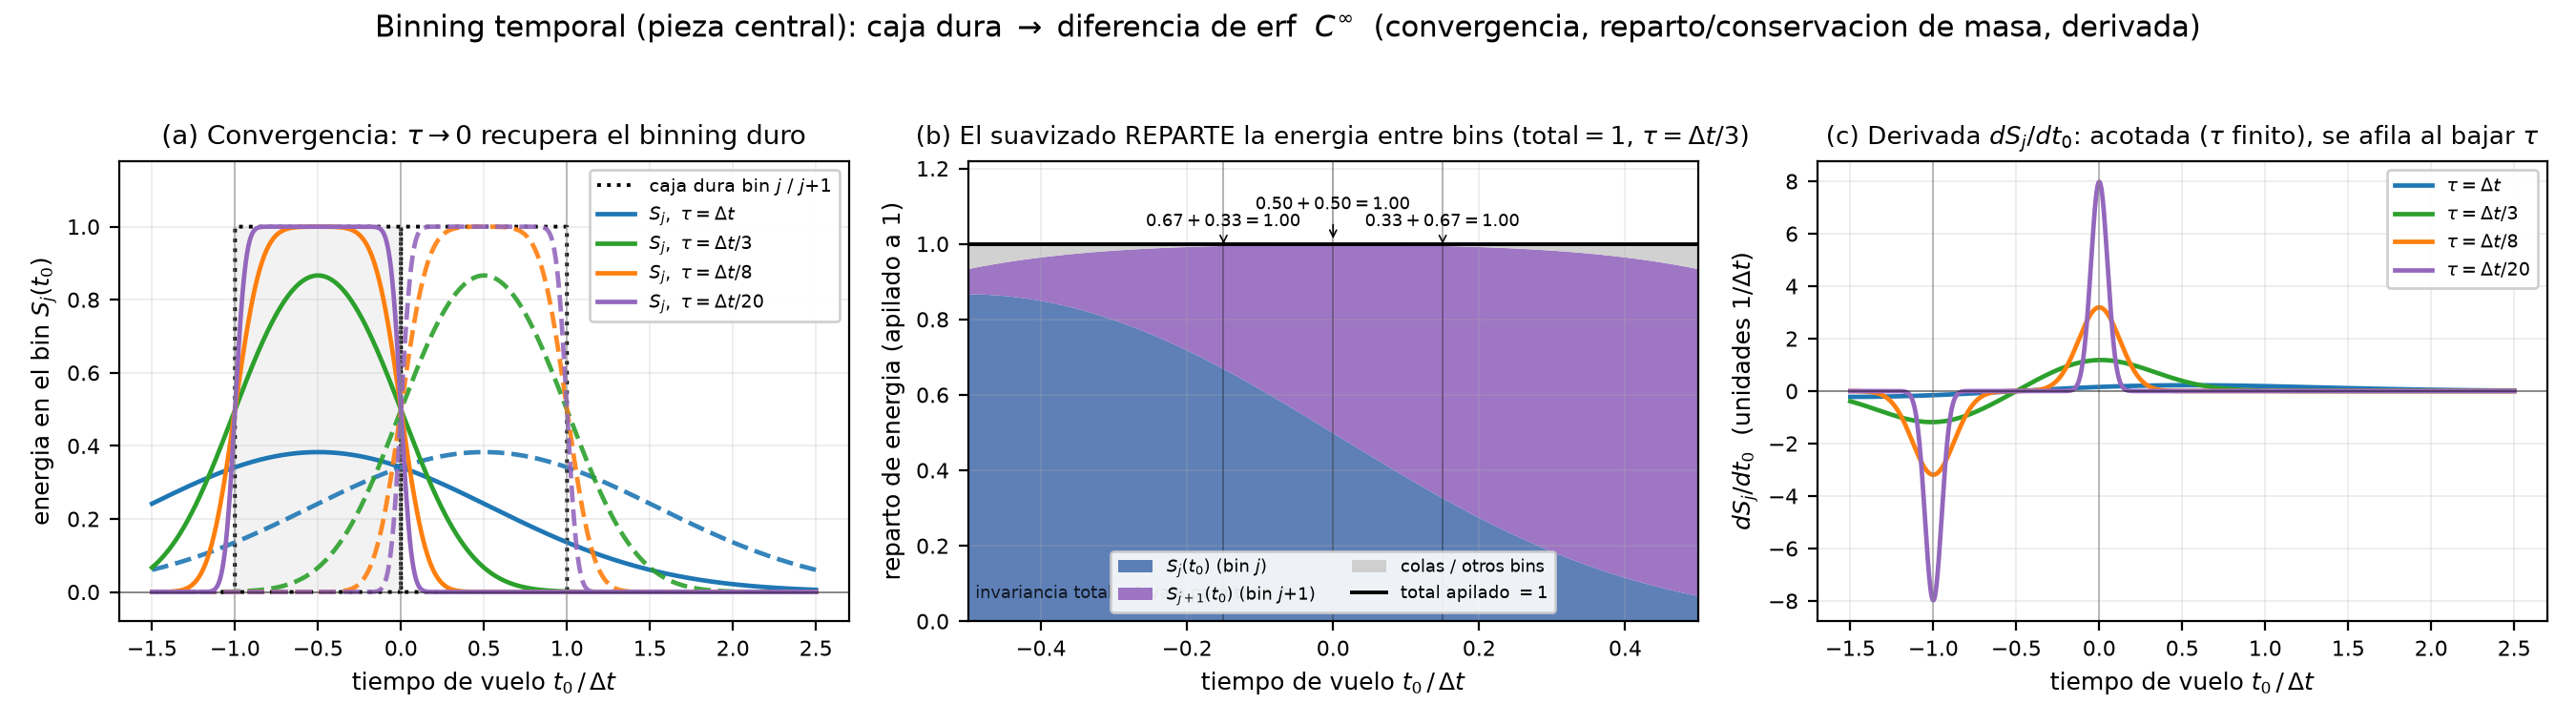
\includegraphics[width=0.9\textwidth]{../plots/crb_smoothing_binning.png}%
}{\textit{(Pendiente: ejecutar \texttt{generate\_smoothing\_plots.py}.)}}
\caption{Binning temporal (paso (i), \emph{pieza central}): caja dura
($\lceil\cdot\rceil$ / Dirac, no derivable) $\to$ diferencia de $\erf$
\eqref{eq:erf-bin} ($C^\infty$), barriendo el ancho de pulso
$\tau\in\{\Delta t,\Delta t/3,\Delta t/8,\Delta t/20\}$ (par\'ametros reales de
\texttt{ForwardConfig}). \textbf{(a) Convergencia:} $S_j(t_0)$ para dos bins
adyacentes $j,j{+}1$; a menor $\tau$ las curvas se pegan a la \emph{caja dura}
(punteada) con flancos casi verticales, y $\tau\to0$ recupera el binning duro.
\textbf{(b) Reparto de energ\'ia (conservaci\'on de masa):} para un pulso
representativo ($\tau=\Delta t/3$), la energ\'ia de \emph{un} pulso se
\emph{reparte} entre los dos bins vecinos como bandas \textbf{apiladas}
($S_j$ abajo, $S_{j+1}$ encima, m\'as una banda fina de colas/otros bins), con
altura total \emph{constante} $=1$; las anotaciones ($0.67{+}0.33{=}1.00$,
$0.50{+}0.50{=}1.00$, $0.33{+}0.67{=}1.00$) muestran la aritm\'etica del reparto
al desplazar $t_0$ sobre el borde compartido. El total $=1$ vale para \emph{todo}
$\tau$ (aunque se dibuje uno): \'este es el criterio de validez, no el parecido
visual. \textbf{(c) Derivada:}
$dS_j/dt_0$ es continua y \textbf{acotada} para $\tau$ finito y \emph{se afila}
(pico $\sim1/\tau$) al bajar $\tau$, ilustrando el \emph{trade-off}
suavidad$\leftrightarrow$fidelidad y por qu\'e el l\'imite duro no es derivable.}
\label{fig:smooth-binning}
\end{figure}

\begin{remark}[\textup{?`}Por qu\'e no llevar $\tau\to0$, $\kappa\to\infty$, $\beta\to\infty$?]
\label{rem:trade-off}
Ser\'ia tentador tomar los par\'ametros de suavizado al l\'imite para ``parecerse
m\'as al simulador''. No conviene, por tres razones:
\begin{itemize}[nosep]
    \item \textbf{El objetivo es \emph{derivar}, y en el l\'imite la derivada se
    rompe.} La derivada del pulso escala como $\sim1/\tau$
    (Fig.~\ref{fig:smooth-binning}(c)) y la de la sigmoide como $\sim\kappa$
    (Prop.~\ref{prop:sigmoid}). Al llevar $\tau\to0$, $\kappa,\beta\to\infty$, el
    pico de la derivada \textbf{diverge} (tiende a deltas), la Fisher
    $\matr I=\matr J^{\mathsf T}\diag(1/\vect g)\,\matr J$ \eqref{eq:fisher} se
    vuelve \textbf{mal condicionada} e inestable, y la rejilla fija ni siquiera
    resuelve transiciones tan finas: se \textbf{recupera el problema no derivable
    original} (Prop.~\ref{prop:fd}). En una frase: m\'as fidelidad $\Rightarrow$
    derivada m\'as salvaje.
    \item \textbf{$\tau$ y $\kappa$ tienen sentido f\'isico.} El pulso l\'aser real
    tiene \textbf{ancho finito} ($\sim\Delta t$) y el borde ocluyente tiene
    \textbf{penumbra finita} ($\sim$ tama\~no de p\'ixel). El $\lceil\cdot\rceil$ y
    el Heaviside del simulador son la \emph{idealizaci\'on cruda}, \textbf{no la
    verdad f\'isica}: un $\tau,\kappa$ finitos son de hecho \emph{m\'as realistas}.
    (Es cierto que ``$\tau\to0$ se parece m\'as al simulador'', pero el
    \texttt{ceil} del simulador no es la f\'isica real.)
    \item \textbf{$\beta$ es m\'as num\'erico.} El \emph{clamp} del coseno s\'i es un
    $\max(0,\cdot)$ real; $\beta$ solo suaviza el codo. Se elige
    \emph{suficientemente grande} para que el redondeo ($\sim1/\beta$) sea
    insignificante salvo pegado a $\cos=0$ ($\beta=50\Rightarrow\sim0.02$,
    min\'usculo frente a $[-1,1]$), pero \textbf{finito} para conservar la
    diferenciabilidad (cota uniforme $(\log2)/\beta$, Prop.~\ref{prop:softplus}).
\end{itemize}
\textbf{Conclusi\'on:} se elige un valor \textbf{intermedio}, que balancea
fidelidad $\leftrightarrow$ derivada acotada / Fisher bien condicionada. El
l\'imite duro se recupera formalmente (Prop.~\ref{prop:consistencia}) pero no es
donde se opera.
\end{remark}

%------------------------------------------------------------------------------
\subsection{(ii) Ocultamiento: de umbral duro a sigmoide de penumbra}
\label{sec:vis}
%------------------------------------------------------------------------------

\textbf{C\'omo estaba.} La m\'ascara dura \eqref{eq:raster-noc},
$\texttt{noc}=\mathbf 1\{\texttt{xint}>0\}$, con \texttt{xint} la coordenada $x$
donde el segmento faceta$\to$p\'ixel cruza $y=0$.

\textbf{Por qu\'e no es derivable.} Es un Heaviside: discontinuo en la frontera
$\{\texttt{xint}=0\}$; derivada cl\'asica $0$ a los lados y delta en la frontera
(Teorema~\ref{thm:ift}).

\textbf{Con qu\'e se reemplaza.} Mantenemos la \emph{misma} funci\'on de borde en
forma cerrada,
\begin{equation}
    d_{\mathrm{edge}}(\vect{\psi},\vect{p}_f)
    =s_x - s_y\,\frac{s_x-p_{f,x}}{s_y-p_{f,y}}
    \;\;(\equiv\texttt{xint}),
    \qquad s_x=\rho\cos\varphi,\ s_y=\rho\sin\varphi,
    \label{eq:dedge}
\end{equation}
y sustituimos el Heaviside por una \textbf{sigmoide log\'istica}
\begin{equation}
    \boxed{\;
    \mathrm{vis}(\vect{\psi},\vect{p}_f)
    =\sigma\!\bigl(\kappa\,d_{\mathrm{edge}}\bigr)
    =\frac{1}{1+e^{-\kappa\, d_{\mathrm{edge}}(\vect{\psi},\vect{p}_f)}}
    \;\in(0,1).
    \;}
    \label{eq:sigmoid}
\end{equation}

\textbf{Por qu\'e esta opci\'on.} La sigmoide es (1) $C^\infty$ y \textbf{acotada}
en $(0,1)$, id\'onea para una ``visibilidad''; (2) \textbf{mon\'otona}, de modo que
no introduce oscilaciones esp\'urias; (3) tiende al Heaviside cuando
$\kappa\to\infty$ (con convergencia uniforme fuera de una capa de ancho
$\sim1/\kappa$, Prop.~\ref{prop:sigmoid}); y (4) tiene \textbf{derivada simple}
$\sigma'=\kappa\,\sigma(1-\sigma)$. El par\'ametro $\kappa$ es el ancho de
\emph{penumbra}: la transici\'on sombra$\to$luz ocurre en una banda de
semi-anchura $\sim1/\kappa$ (metros). Por defecto $\kappa=60$, i.e.\ penumbra
$\sim1/\kappa=1.67$\,cm. \textbf{Advertencia:} con la rejilla del simulador el
paso de p\'ixel es $0.25/64=0.39$\,cm, de modo que esa penumbra abarca
$\sim4.3$ p\'ixeles: es un ancho \textbf{gen\'erico, m\'as grueso} que la
discretizaci\'on real. Este es un suavizado deliberadamente conservador de la
rama (a)+(b); parte del desajuste de \emph{forma} con el FD proviene de aqu\'i
(Sec.~\ref{sec:resultados}). La rama (a)+(b)+(c) ata los anchos a la
discretizaci\'on: $\kappa=256$ ($1/\kappa=$ un p\'ixel) y $\tau=\Delta t/\sqrt{12}$
(desviaci\'on de un bin uniforme).

\begin{figure}[ht]
\centering
\IfFileExists{../plots/crb_smoothing_occlusion.png}{%
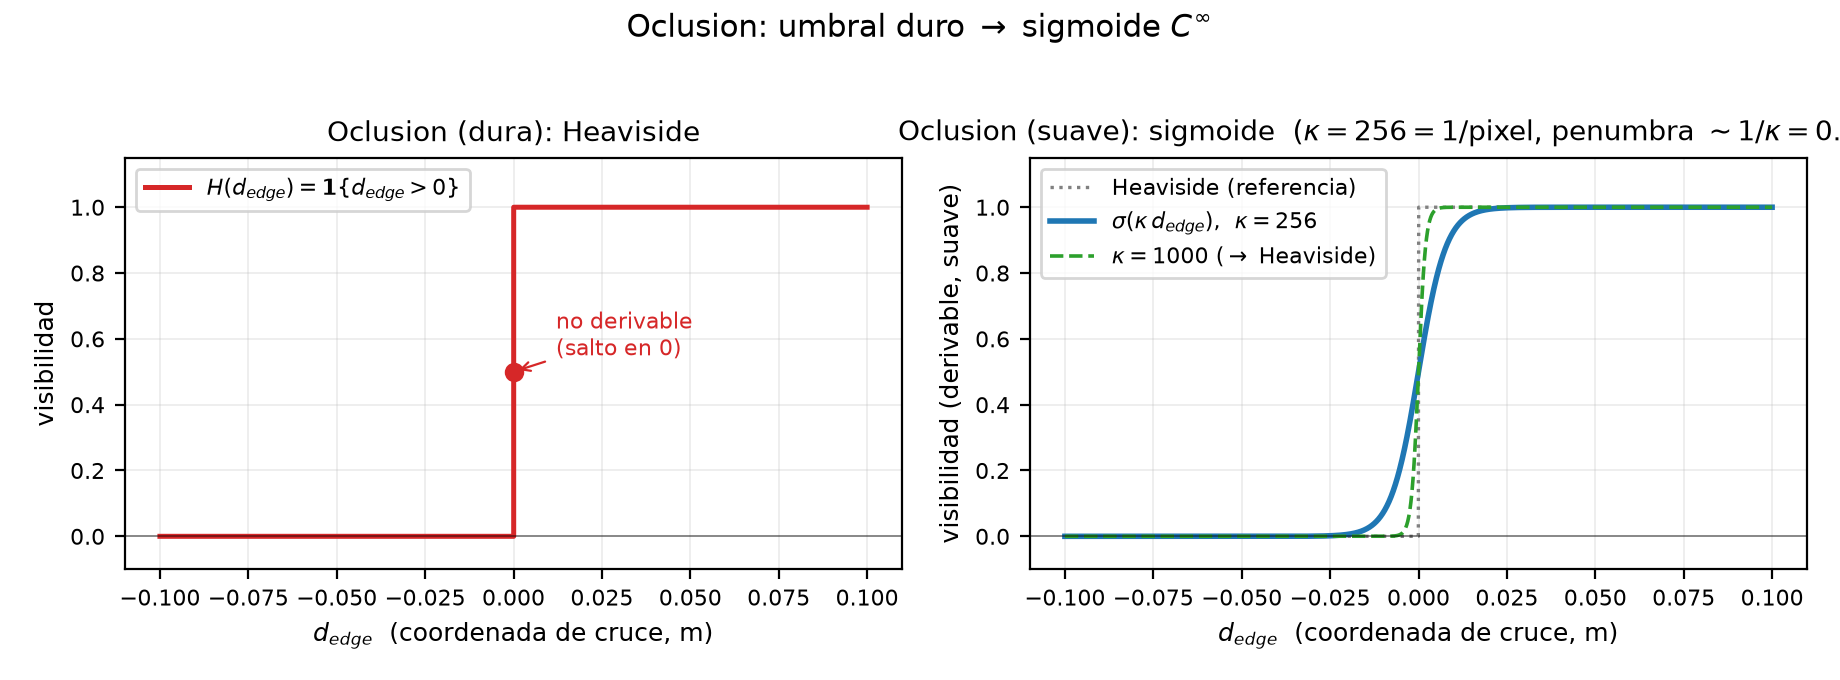
\includegraphics[width=0.9\textwidth]{../plots/crb_smoothing_occlusion.png}%
}{\textit{(Pendiente: ejecutar \texttt{generate\_smoothing\_plots.py}.)}}
\caption{Ocultamiento (paso (ii)). \textbf{Izquierda:} funci\'on \textbf{no
derivable} (dura): el Heaviside $\mathbf 1\{d_{\mathrm{edge}}>0\}$, con salto en
$d_{\mathrm{edge}}=0$. \textbf{Derecha:} su \textbf{reemplazo suave}, la sigmoide
$\sigma(\kappa\,d_{\mathrm{edge}})$ \eqref{eq:sigmoid} con $\kappa=60$ (penumbra
$\sim1/\kappa$); una segunda curva con $\kappa=200$ sugiere el l\'imite
$\kappa\to\infty$ (Heaviside punteado de referencia). Par\'ametro real de
\texttt{ForwardConfig}.}
\label{fig:smooth-occlusion}
\end{figure}

%------------------------------------------------------------------------------
\subsection{(iii) \emph{Clamps}: de \texorpdfstring{$\max(0,\cdot)$}{max(0,.)} a \emph{softplus}}
\label{sec:softplus}
%------------------------------------------------------------------------------

\textbf{C\'omo estaba.} Cada uno de los cuatro cosenos de \eqref{eq:raster-cos}
pasa por $[\,c_k\,]_+=\max(0,c_k)$ (una cara que no ``ve'' aporta $0$).

\textbf{Por qu\'e no es derivable.} $\max(0,\cdot)$ es continuo y Lipschitz, pero
tiene un \textbf{codo} en $c_k=0$: derivadas laterales $0\neq1$
(Prop.~\ref{prop:relu}).

\textbf{Con qu\'e se reemplaza.} Por la \textbf{\emph{softplus}}
\begin{equation}
    \softplus_\beta(x)=\frac{1}{\beta}\log\!\bigl(1+e^{\beta x}\bigr),
    \qquad
    \softplus_\beta(x)\xrightarrow[\beta\to\infty]{}\max(0,x),
    \label{eq:softplus}
\end{equation}
aplicada a los cuatro cosenos \emph{crudos} $c_1,\dots,c_4$ (los argumentos de
\eqref{eq:raster-cos} sin el $[\cdot]_+$):
\begin{equation}
    c_1=\frac{\hat{\vect n}_s\!\cdot\!(\vect{p}_l-\vect{p}_s)}{d_1},\;\;
    c_2=\frac{\hat{\vect n}_s\!\cdot\!(\vect{p}_f-\vect{p}_s)}{d_2},\;\;
    c_3=\frac{\hat{\vect n}_l\!\cdot\!(\vect{p}_s-\vect{p}_l)}{d_1},\;\;
    c_4=\frac{\hat{\vect n}_f\!\cdot\!(\vect{p}_s-\vect{p}_f)}{d_2},
    \label{eq:cos-crudos}
\end{equation}
\begin{equation}
    f_{\mathrm{smooth}}(\vect{\psi},\vect{p}_f)
    =\prod_{k=1}^{4}\softplus_\beta\!\bigl(c_k(\vect{\psi},\vect{p}_f)\bigr).
    \label{eq:f-smooth}
\end{equation}

\textbf{Por qu\'e esta opci\'on.} La softplus (1) es $C^\infty$; (2)
$\to\max(0,\cdot)$ con \textbf{cota uniforme} $0\le\softplus_\beta-\max(0,\cdot)\le
(\log2)/\beta$ para \emph{todo} $x$ (Prop.~\ref{prop:softplus}), lo que controla
el sesgo del suavizado de forma expl\'icita e independiente del punto; y (3) tiene
\textbf{derivada} exactamente la sigmoide $\softplus_\beta'=\sigma_\beta\in(0,1)$,
lo que encadena de forma natural con el resto. El codo se suaviza en una escala
$\sim1/\beta$; por defecto $\beta=50$ (ancho $\sim0.02$). Las distancias
$\norm{\cdot}=\sqrt{\langle\cdot,\cdot\rangle}$ ya son $C^\infty$ mientras no se
anulen (garantizado por $\vect{p}_s\neq\vect{p}_l,\vect{p}_f$).

\begin{figure}[ht]
\centering
\IfFileExists{../plots/crb_smoothing_foreshortening.png}{%
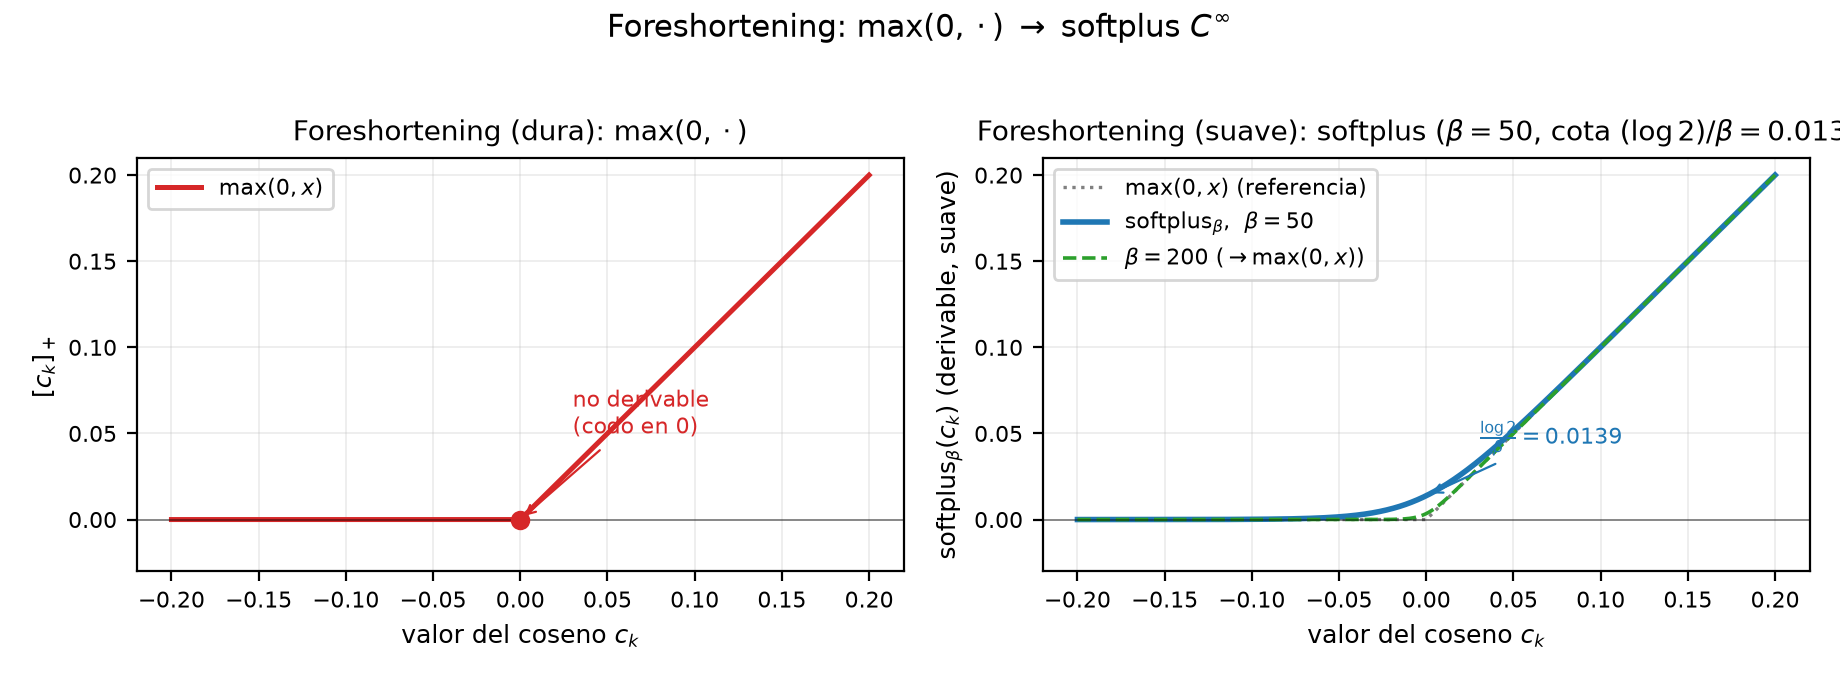
\includegraphics[width=0.9\textwidth]{../plots/crb_smoothing_foreshortening.png}%
}{\textit{(Pendiente: ejecutar \texttt{generate\_smoothing\_plots.py}.)}}
\caption{\emph{Foreshortening} (paso (iii)). \textbf{Izquierda:} funci\'on
\textbf{no derivable} (dura): el \emph{clamp} $\max(0,c_k)$, con codo no derivable
en $c_k=0$. \textbf{Derecha:} su \textbf{reemplazo suave}, la
$\softplus_\beta(c_k)$ \eqref{eq:softplus} con $\beta=50$; se anota la cota
uniforme $(\log2)/\beta$ (Prop.~\ref{prop:softplus}) y una segunda curva con
$\beta=200$ sugiere el l\'imite $\beta\to\infty$ ($\max(0,\cdot)$ punteado de
referencia). Par\'ametro real de \texttt{ForwardConfig}.}
\label{fig:smooth-foreshortening}
\end{figure}

%------------------------------------------------------------------------------
\subsection{(iv) Ensamblado de \texorpdfstring{$g(\vect{\psi})=A\,S+b$}{g = A S + b}}
\label{sec:ensamble}
%------------------------------------------------------------------------------

Reuniendo \eqref{eq:erf-bin}, \eqref{eq:sigmoid} y \eqref{eq:f-smooth}, con la
ca\'ida radial \textbf{$4\pi^2$ del simulador} (\textbf{no} $8\pi^3$) y
\textbf{cuatro} cosenos (\textbf{no} cinco), la tasa esperada en la medici\'on
$q=(i,j)$ es el producto
\begin{equation}
    \boxed{\;
    y_q(\vect{\psi})
    =
    \underbrace{\frac{I_{\mathrm{laser}}\,(w\,h)\;\mathrm{vis}(\vect{\psi},\vect{p}_{f,i})\,
                      f_{\mathrm{smooth}}(\vect{\psi},\vect{p}_{f,i})}
                     {4\pi^2\,\norm{\vect{p}_s-\vect{p}_l}^2\,
                      \norm{\vect{p}_s-\vect{p}_{f,i}}^2}}
                     _{\textstyle A_i(\vect{\psi})\ \text{(amplitud espacial)}}
    \;\cdot\;
    \underbrace{S_j(\vect{\psi})}_{\textstyle \text{pulso en el bin}} ,
    \;}
    \label{eq:yq-smooth}
\end{equation}
\begin{equation}
    g_q(\vect{\psi}) = y_q(\vect{\psi}) + b,\qquad b=0.1 .
    \label{eq:g-smooth}
\end{equation}

\begin{remark}[Amplitud f\'isica: \'area $w\!\cdot\!h$ e \texttt{laser\_intensity} reales]
\label{rem:area}
En el simulador el \'area $A$ \emph{var\'ia por tri\'angulo}, pero la suma de las
\'areas de los tri\'angulos que teselan la faceta es exactamente $w\,h$
(ancho\,$\times$\,alto). En el forward de faceta \emph{puntual} no hay malla, de
modo que usamos una \textbf{\'unica \'area f\'isica} $A_{\mathrm{eff}}=w\,h$ (con
$w=0.5$\,m fijo y $h$ el par\'ametro de altura) y la \textbf{intensidad real} del
simulador $I_{\mathrm{laser}}=1000$; ya \textbf{no} hay ganancia arbitraria $G$
($\alpha$ es un albedo opcional fijado a $1$). Esto es la \textbf{variante (a)}:
pone la \emph{escala f\'isica correcta} (unidades del rasterizador) --- la
amplitud escala con $h$ como lo hace la malla --- de modo que el CRB anal\'itico y
el FD quedan en las \textbf{mismas unidades} (Sec.~\ref{sec:resultados}).
\textbf{Pero no coinciden}: usar una \'unica evaluaci\'on en el centroide es una
\textbf{cuadratura de un punto} de la integral de malla, y su error es
\textbf{sistem\'atico}, no un residual que se anule al afinar el suavizado. En
concreto, la faceta real de $0.5\times1$\,m tiene una parte \emph{ocluida} para
muchos p\'ixeles mientras su centroide sigue siendo visible, de modo que el punto
\textbf{sobreestima} la energ\'ia ($\sim1.5\times$ frente a la suma de malla;
tambi\'en por la no linealidad de $1/d_2^2$ y de los cuatro cosenos sobre la
faceta extendida). Al endurecer ($\tau\to0$, $\beta,\kappa\to\infty$) esta
variante converge a su \textbf{propio} forward duro \emph{puntual}, \textbf{no} al
de malla del simulador. La correcci\'on de este sesgo es la \textbf{suma sobre
malla} (rama (a)+(b)+(c)), no reducir el suavizado.
\end{remark}

El fondo $b>0$ mantiene $1/g_q$ finito \textbf{sin} piso $\varepsilon$ artificial.
Cada factor de \eqref{eq:yq-smooth} es $C^\infty$ en $\vect{\psi}=(\rho,\varphi,h)$
(se prueba en la Sec.~\ref{sec:justificacion}), luego $g_q$ lo es. Implementado en
\texttt{crb\_analytic\_forward.py} (clase \texttt{AnalyticForwardModel}; ver
\texttt{ForwardConfig} para $I_{\mathrm{laser}},w,\alpha,b,\beta,\kappa,\tau$ y la
geometr\'ia fija de la rejilla del simulador $64\times64$). La posici\'on de
c\'amara $\vect{p}_c$ \textbf{no} aparece: el forward es de dos rebotes.

%==============================================================================
\section{La derivada anal\'itica (paso a paso)}
\label{sec:derivadas}
%==============================================================================

Ahora que $g_q\in C^\infty$, obtenemos $\partial g_q/\partial\rho$,
$\partial g_q/\partial\varphi$, $\partial g_q/\partial h$ en forma cerrada. Como
$g_q=y_q+b$ y $b$ no depende de $\vect{\psi}$,
$\partial g_q/\partial\psi_m=\partial y_q/\partial\psi_m$.

\paragraph{Paso 1: regla del producto.} Por la estructura $y_q=A_i\,S_j$ de
\eqref{eq:yq-smooth},
\begin{equation}
    \frac{\partial y_q}{\partial\psi_m}
    =\frac{\partial A_i}{\partial\psi_m}\,S_j
    +A_i\,\frac{\partial S_j}{\partial\psi_m},
    \qquad \psi_m\in\{\rho,\varphi,h\}.
    \label{eq:chain}
\end{equation}

\paragraph{Paso 2: derivadas de los bloques.} Cada bloque suave aporta una
derivada elemental bien definida en todo el dominio:
\begin{align}
    \frac{\partial S_j}{\partial\psi_m}
    &=-\,\frac{\partial t_0}{\partial\psi_m}\,
    \frac{1}{\tau\sqrt{2\pi}}
    \left[
        e^{-(t^{(j)}_{\mathrm{hi}}-t_0)^2/2\tau^2}
        -e^{-(t^{(j)}_{\mathrm{lo}}-t_0)^2/2\tau^2}
    \right],
    \label{eq:dS}\\[4pt]
    \frac{d}{dx}\,\softplus_\beta(x)&=\sigma(\beta x),
    \qquad
    \frac{d}{dx}\,\sigma(\kappa x)=\kappa\,\sigma(\kappa x)\bigl(1-\sigma(\kappa x)\bigr),
    \label{eq:dblocks}
\end{align}
donde \eqref{eq:dS} sale de derivar \eqref{eq:erf-bin} con
$\erf'(z)=\tfrac{2}{\sqrt\pi}e^{-z^2}$.

\paragraph{Paso 3: derivadas geom\'etricas.} $\partial t_0/\partial\psi_m$ se
obtiene de \eqref{eq:tof} derivando las dos normas: para $\vect r=\vect p_s-\vect
p_\bullet$,
\begin{equation}
    \frac{\partial\norm{\vect r}}{\partial\psi_m}
    =\frac{\vect r\cdot\partial_{\psi_m}\vect p_s}{\norm{\vect r}},
    \qquad
    \partial_\rho\vect p_s=(\cos\varphi,\sin\varphi,0),\;\;
    \partial_\varphi\vect p_s=(-\rho\sin\varphi,\rho\cos\varphi,0),\;\;
    \partial_h\vect p_s=(0,0,\tfrac12),
    \label{eq:dnorm}
\end{equation}
y las derivadas de los cosenos \eqref{eq:cos-crudos} y de $\mathrm{vis}$ salen por
regla de la cadena con \eqref{eq:dblocks} y \eqref{eq:dnorm}. La derivada del
producto de cuatro \emph{softplus} se propaga con la regla del producto.

\paragraph{Paso 4: generaci\'on simb\'olica.} En la pr\'actica \textbf{no}
escribimos esto a mano: se genera con \texttt{sympy} (\texttt{sp.diff}, an\'alogo
directo al Mathematica del \emph{writeup}) y se compila a
\texttt{numpy}/\texttt{scipy} con \texttt{lambdify} para evaluaci\'on vectorizada
sobre toda la rejilla $(i,j)$:
\begin{lstlisting}
# crb_analytic_forward.py  (construccion simbolica, resumida)
rho, phi, h = sp.symbols("rho phi h", real=True)
ps = sp.Matrix([rho*sp.cos(phi), rho*sp.sin(phi), h/2])  # centroide en z=h/2
ns = sp.Matrix([-sp.cos(phi), -sp.sin(phi), 0])
d1, d2 = (ps-pl).norm(), (ps-pf).norm()               # dos rebotes: C-inf
softplus = lambda x: sp.log(1 + sp.exp(beta*x))/beta   # (iii)
c1 = ns.dot(pl-ps)/d1;  c2 = ns.dot(pf-ps)/d2          # cuatro cosenos (dot1..dot4)
c3 = nl.dot(ps-pl)/d1;  c4 = nf.dot(ps-pf)/d2
f_fore = softplus(c1)*softplus(c2)*softplus(c3)*softplus(c4)
d_edge = sx - sy*(sx-px)/(sy-py)                        # (ii)
vis     = 1/(1 + sp.exp(-kappa*d_edge))
t0 = (d1 + d2)/c                                        # (i)
S  = (sp.erf((thi-t0)/(sp.sqrt(2)*tau))
      - sp.erf((tlo-t0)/(sp.sqrt(2)*tau)))/2
area_eff = w*h                                          # (a) area fisica w*h
y  = alpha*laser_intensity*area_eff*vis*f_fore/(4*sp.pi**2*d1**2*d2**2) * S  # 4*pi^2, NO 8*pi^3
dy_drho = sp.diff(y, rho)      # derivadas CERRADAS
dy_dphi = sp.diff(y, phi)
dy_dh   = sp.diff(y, h)
f_dy = sp.lambdify((rho,phi,h,px,py,tlo,thi), dy_drho, modules=["scipy","numpy"])
\end{lstlisting}
Las funciones expuestas son \texttt{analytic\_forward\_g(psi,\dots)},
\texttt{analytic\_jacobian\_g(psi,\dots)} y \texttt{compute\_crb\_analytic(psi,\dots)}.

%==============================================================================
\section{Justificaci\'on matem\'atica (paso a paso)}
\label{sec:justificacion}
%==============================================================================

Esta secci\'on desarrolla, con el aparato del an\'alisis real y \textbf{paso a
paso}, \emph{por qu\'e} el forward duro del simulador
\eqref{eq:raster-int}--\eqref{eq:xint} no admite un gradiente cl\'asico
informativo y \emph{c\'omo} la construcci\'on de la Sec.~\ref{sec:construccion}
produce una funci\'on $C^\infty$ con derivadas exactas. Cada enunciado se refiere a
los bloques \emph{del simulador} (los cuatro cosenos, la \texttt{xint} real, el
\texttt{ceil}).

%------------------------------------------------------------------------------
\subsection*{Paso 0. Preliminares y el forward duro}
\label{sec:prelim}
%------------------------------------------------------------------------------

Sea $\vect{\psi}=(\rho,\varphi,h)$ (o $(\rho,\varphi)$ fijando $h$) en el dominio
de par\'ametros
\begin{equation}
    \Theta=\bigl\{(\rho,\varphi,h)\in\R^3 : \rho>0,\ \varphi\in(0,\pi),\ h>0\bigr\},
    \label{eq:Theta}
\end{equation}
un \textbf{abierto} de $\R^3$. La faceta puntual es
$\vect{p}_s(\vect{\psi})=(\rho\cos\varphi,\rho\sin\varphi,h/2)$ (centroide a media
altura, \eqref{eq:pose}); el l\'aser $\vect{p}_l$ y los p\'ixeles de piso
$\{\vect{p}_{f,i}\}_{i=1}^{P}$ son \emph{fijos}. El espacio de mediciones es $\R^N$, $q=(i,j)$ con $i$ p\'ixel y $j$
bin $[t_{j-1},t_j]$, $t_j=j\,\Delta t$.

\begin{assumption}[No degeneraci\'on geom\'etrica]\label{as:geom}
Para todo $\vect{\psi}\in\Theta$ y todo p\'ixel $i$:
(a) $\vect{p}_s(\vect{\psi})\neq\vect{p}_l$ y
$\vect{p}_s(\vect{\psi})\neq\vect{p}_{f,i}$ (las dos distancias $d_1,d_2$ son
estrictamente positivas);
(b) $s_y(\vect{\psi})\neq p_{f,y,i}$, de modo que la coordenada de cruce
\eqref{eq:xint} est\'a bien definida. Si hiciera falta, restringimos $\Theta$ a
un abierto donde (a)--(b) se cumplan.
\end{assumption}

Con $d_i(\vect{\psi})=\norm{\vect{p}_s-\vect{p}_l}+\norm{\vect{p}_s-\vect{p}_{f,i}}$
el camino de dos rebotes y $t_{0,i}(\vect{\psi})=d_i(\vect{\psi})/c$, el forward
\textbf{duro} del simulador se escribe formalmente
\begin{equation}
    y^{\mathrm{hard}}_q(\vect{\psi})
    =A_i(\vect{\psi})\;
    \mathbf{1}_{[t_{j-1},t_j)}\!\bigl(t_{0,i}(\vect{\psi})\bigr)\;
    \mathbf{1}_{\{e_i(\vect{\psi})>0\}},
    \qquad g^{\mathrm{hard}}_q=y^{\mathrm{hard}}_q+b,
    \label{eq:hard}
\end{equation}
donde $A_i\ge0$ es la amplitud radiom\'etrica (producto de \textbf{cuatro}
cosenos con \emph{clamp} y ca\'ida $1/(4\pi^2 d_1^2 d_2^2)$), $e_i=\texttt{xint}$
la funci\'on de borde \eqref{eq:xint}, y $\mathbf 1_S$ la indicatriz. El primer
indicador codifica el \texttt{ceil}; el segundo, el ocultamiento; los cuatro
\emph{clamps} viven dentro de $A_i$. \'Estas son las tres operaciones de la
Obs.~\ref{rem:tres}.

%------------------------------------------------------------------------------
\subsection*{Paso 1. Los bloques ``suaves'' del simulador ya son \texorpdfstring{$C^\infty$}{C-inf}}
\label{sec:reg-suaves}
%------------------------------------------------------------------------------

\begin{lemma}[La norma eucl\'idea es $C^\infty$ fuera del origen]\label{lem:norm}
$\norm{\cdot}:\R^n\setminus\{0\}\to\R$, $x\mapsto\sqrt{x\cdot x}$, es $C^\infty$
(de hecho real-anal\'itica).
\end{lemma}
\begin{proof}
$x\mapsto x\cdot x$ es un polinomio ($C^\infty$) y positivo en
$\R^n\setminus\{0\}$; $\sqrt{\cdot}$ es $C^\infty$ en $(0,\infty)$; la
composici\'on es $C^\infty$.
\end{proof}

\begin{proposition}[Distancias y tiempo de vuelo $C^\infty$]\label{prop:dist}
Bajo la Hip.~\ref{as:geom}(a), para cada $i$ las funciones $d_1,d_2,d_i,t_{0,i}$
son $C^\infty$ en $\Theta$.
\end{proposition}
\begin{proof}
Cada componente de $\vect{p}_s=(\rho\cos\varphi,\rho\sin\varphi,h/2)$ es
producto/composici\'on de $\rho,\cos,\sin$ (real-anal\'iticas), luego
$\vect{p}_s\in C^\infty$. Las traslaciones por $\vect{p}_l,\vect{p}_{f,i}$ son
afines. Por la Hip.~\ref{as:geom}(a) los argumentos no se anulan, as\'i que el
Lema~\ref{lem:norm} y la cadena dan $\norm{\vect{p}_s-\vect{p}_l},
\norm{\vect{p}_s-\vect{p}_{f,i}}\in C^\infty$; su suma $d_i$ y $t_{0,i}=d_i/c$
tambi\'en.
\end{proof}

\begin{proposition}[Los cuatro cosenos son $C^\infty$]\label{prop:cos}
Cada coseno crudo $c_k$ de \eqref{eq:cos-crudos},
$k=1,\dots,4$, es $C^\infty$ en $\Theta$.
\end{proposition}
\begin{proof}
La normal $\hat{\vect n}_s=(-\cos\varphi,-\sin\varphi,0)$ es $C^\infty$;
$\hat{\vect n}_l,\hat{\vect n}_f$ son constantes. Los vectores $\vect p_l-\vect
p_s$, $\vect p_f-\vect p_s$ (y sus opuestos) son $C^\infty$; el numerador
$\hat{\vect n}\!\cdot\!\vect u$ es bilineal en entradas $C^\infty$; el denominador
$d_1$ o $d_2$ es $C^\infty$ y no nulo (Hip.~\ref{as:geom}(a),
Prop.~\ref{prop:dist}). El cociente con denominador no nulo es $C^\infty$.
\end{proof}

As\'i, la amplitud $A_i$ \emph{sin} los \emph{clamps} y sin la indicatriz de
ocultamiento ya ser\'ia $C^\infty$ (la ca\'ida $1/(4\pi^2 d_1^2 d_2^2)$ es
rec\'iproca de un producto de normas $C^\infty$ positivas). \textbf{Toda} la no
diferenciabilidad viene de los tres operadores duros de \eqref{eq:hard}.

%------------------------------------------------------------------------------
\subsection*{Paso 2. Diagn\'ostico de la no diferenciabilidad}
\label{sec:diagnostico}
%------------------------------------------------------------------------------

\subsubsection*{(a) Los indicadores \texttt{ceil} y \texttt{xint}$>0$: discontinuidad de salto}

\begin{theorem}[Superficie de salto v\'ia funci\'on impl\'icita]\label{thm:ift}
Sea $\phi\in C^1(\Theta)$ (p.\,ej.\ $\phi=t_{0,i}$ para el binning, o
$\phi=e_i$ para el ocultamiento) y $a\in\R$ con
$Z_a:=\{\phi=a\}\neq\varnothing$. Si $\nabla\phi(\vect{\psi}^\ast)\neq\vect 0$ en
$\vect{\psi}^\ast\in Z_a$, entonces cerca de $\vect{\psi}^\ast$ el conjunto $Z_a$
es una hipersuperficie $C^1$ (codimensi\'on $1$), la funci\'on
$\vect{\psi}\mapsto\mathbf{1}_{\{\phi>a\}}$ es \textbf{discontinua} en cada punto
de $Z_a$ y \textbf{localmente constante} (gradiente cl\'asico nulo) en
$\Theta\setminus\phi^{-1}(\{a\})$.
\end{theorem}
\begin{proof}
Alguna $\partial_{\psi_r}\phi(\vect{\psi}^\ast)\neq0$; el \textbf{Teorema de la
funci\'on impl\'icita} despeja $\psi_r$ como funci\'on $C^1$ de las dem\'as cerca de
$\vect{\psi}^\ast$, cuyo grafo es $Z_a$: una hipersuperficie $C^1$. Por
continuidad, $\{\phi>a\}$ y $\{\phi<a\}$ son abiertos donde
$\mathbf 1_{\{\phi>a\}}$ vale $1$ o $0$ (localmente constante, gradiente $\vect
0$). En $Z_a$ todo entorno contiene puntos de ambos lados ($\nabla\phi\neq0$),
luego $\mathbf 1_{\{\phi>a\}}$ salta.
\end{proof}

Aplicado a \eqref{eq:hard}: el binning $\mathbf
1_{[t_{j-1},t_j)}(t_{0,i}(\vect{\psi}))$ salta a trav\'es de las
\textbf{isocronas} $\{t_{0,i}=t_{j-1}\}$, $\{t_{0,i}=t_j\}$; y el ocultamiento
$\mathbf 1_{\{e_i>0\}}$ salta a trav\'es de la \textbf{frontera de sombra}
$\{e_i=0\}$ (la $\texttt{xint}=0$ real). Entre saltos, ambos son localmente
constantes: la patolog\'ia ``\textbf{meseta plana} ($\nabla=\vect0$) $+$
\textbf{salto}'', que borra la informaci\'on de primer orden salvo en un conjunto
de medida nula donde ni existe la derivada.

\subsubsection*{(b) \emph{Clamp} $\max(0,\cdot)$: convexo, Lipschitz, no derivable en $0$}

\begin{proposition}[Regularidad de $\max(0,\cdot)$]\label{prop:relu}
$r(x)=\max(0,x)$ es convexa y $1$-Lipschitz en $\R$, derivable en
$\R\setminus\{0\}$ con $r'(x)=\mathbf{1}_{\{x>0\}}$, y \emph{no} derivable en $0$:
$r'_-(0)=0\neq1=r'_+(0)$.
\end{proposition}
\begin{proof}
$r=\max\{0,x\}$ es m\'aximo puntual de afines, luego convexo; tiene pendiente $0$
o $1$, luego $1$-Lipschitz. Para $x\neq0$ coincide localmente con $0$ o $x$. En
$0$: $r'_+(0)=\lim_{t\downarrow0}t/t=1$, $r'_-(0)=\lim_{t\uparrow0}0/t=0$; difieren.
\end{proof}

\begin{theorem}[Rademacher]\label{thm:rademacher}
Si $f:\R^n\to\R$ es localmente Lipschitz, es diferenciable en casi todo punto
(medida de Lebesgue).
\end{theorem}

La Prop.~\ref{prop:relu} y el Teorema~\ref{thm:rademacher} sit\'uan los cuatro
\emph{clamps} en ``Lipschitz $\Rightarrow$ derivable c.t.p.'': su \'unico defecto
es un conjunto \emph{numerable} de codos. En cambio los indicadores de
\eqref{eq:hard} \textbf{no son Lipschitz} (saltan): est\'an \emph{fuera} de
Rademacher, son \textbf{discontinuos}.

\subsubsection*{(c) Derivada distribucional y fracaso de las diferencias finitas}

En sentido distribucional $H'=\delta$ en $\mathcal{D}'(\R)$: la informaci\'on de
primer orden del salto se concentra en un punto de medida nula, mientras la
derivada cl\'asica es $0$ c.t.p. De ah\'i que una diferencia finita sobre un
escal\'on \textbf{no converja}.

\begin{proposition}[Inconsistencia de la diferencia finita en un salto]\label{prop:fd}
Sea $f(x)=A\,\mathbf{1}_{\{x>0\}}$ con $A\neq0$ y la diferencia central
$D_\delta f(x_0)=\frac{f(x_0+\delta)-f(x_0-\delta)}{2\delta}$. Entonces
$D_\delta f(x_0)=A/(2\delta)$ si $\abs{x_0}<\delta$ y $0$ si $\abs{x_0}>\delta$.
En $x_0=0$, $D_\delta f(0)=A/(2\delta)\to\pm\infty$ cuando $\delta\to0^+$; el
l\'imite no existe en el salto y \emph{depende del paso} $\delta$.
\end{proposition}
\begin{proof}
Si $\abs{x_0}>\delta$, $x_0\pm\delta$ caen del mismo lado de $0$, luego
$D_\delta f=0$. Si $\abs{x_0}<\delta$, $x_0-\delta<0<x_0+\delta$ y
$D_\delta f=A/(2\delta)$. Los l\'imites son inmediatos.
\end{proof}

\'Esta es la raz\'on de fondo por la que el pipeline con FD debe afinar
$\delta_\rho,\delta_\varphi,\delta_h$: sobre las mesetas obtiene $0$; cerca de una
isocrona o de la frontera $\texttt{xint}=0$, un valor $\propto1/\delta$.

%------------------------------------------------------------------------------
\subsection*{Paso 3. Herramientas de an\'alisis real}
\label{sec:herramientas}
%------------------------------------------------------------------------------

\begin{lemma}[Convergencia dominada, TCD]\label{lem:tcd}
Si $f_n\to f$ en c.t.p.\ y $\abs{f_n}\le G\in L^1(\mu)$, entonces $f\in L^1$ y
$\int f_n\to\int f$.
\end{lemma}

\begin{theorem}[Derivaci\'on bajo la integral, Leibniz v\'ia TCD]\label{thm:leibniz}
Sea $\Theta\subseteq\R^m$ abierto y $F:\Theta\times X\to\R$ con (i)
$F(\vect{\psi},\cdot)\in L^1$; (ii) $\vect{\psi}\mapsto F(\vect{\psi},t)$
derivable en $\psi_m$ para c.t.\ $t$; (iii) existe $G\in L^1$ y un entorno $U$ de
$\vect{\psi}_0$ con $\abs{\partial_{\psi_m}F(\vect{\psi},t)}\le G(t)$ en $U$.
Entonces $\Phi(\vect{\psi})=\int_X F\,d\mu$ es derivable en $\vect{\psi}_0$ y
$\partial_{\psi_m}\Phi=\int_X\partial_{\psi_m}F\,d\mu$; si $\partial_{\psi_m}F$ es
continua en $\vect{\psi}$, $\Phi\in C^1$.
\end{theorem}
\begin{proof}[Idea]
Al cociente incremental se aplica el TVM,
$\frac{F(\vect{\psi}_0+h_n\vect e_m,t)-F(\vect{\psi}_0,t)}{h_n}
=\partial_{\psi_m}F(\vect{\xi}_n,t)$, dominado por $G$ (iii); el
Lema~\ref{lem:tcd} pasa el l\'imite bajo la integral.
\end{proof}

\begin{theorem}[\emph{Mollifiers} / aproximaci\'on de la identidad]\label{thm:mollifier}
Sea $\eta\in C_c^\infty(\R^n)$, $\eta\ge0$, $\int\eta=1$,
$\eta_\varepsilon(x)=\varepsilon^{-n}\eta(x/\varepsilon)$. Para $f\in
L^1_{loc}$: (a) $f*\eta_\varepsilon\in C^\infty$ y
$\partial^\alpha(f*\eta_\varepsilon)=f*\partial^\alpha\eta_\varepsilon$;
(b) $f*\eta_\varepsilon\to f$ en $L^1_{loc}$ y en c.t.\ punto;
(c) si $f$ es continua en un compacto $K$, la convergencia es \textbf{uniforme}
en $K$.
\end{theorem}
\begin{proof}[Idea]
(a) los cocientes incrementales derivan sobre $\eta_\varepsilon\in C_c^\infty$ e
intercambian con la integral por el Teorema~\ref{thm:leibniz}. (b)--(c) por
$\int\eta_\varepsilon=1$ y concentraci\'on del soporte, usando continuidad $L^1$
de las traslaciones.
\end{proof}

\begin{remark}[N\'ucleo gaussiano]
El n\'ucleo $\rho_\tau(t)=(\tau\sqrt{2\pi})^{-1}e^{-t^2/2\tau^2}$ no tiene soporte
compacto pero es de Schwartz y una aproximaci\'on de la identidad
($\rho_\tau\ge0$, $\int\rho_\tau=1$); valen (a)--(c) del
Teorema~\ref{thm:mollifier} (la dominaci\'on usa el decaimiento gaussiano). Es el
n\'ucleo del pulso \eqref{eq:pulse}.
\end{remark}

\begin{lemma}[$\erf$ es real-anal\'itica]\label{lem:erf}
$\erf(x)=\frac{2}{\sqrt\pi}\int_0^x e^{-u^2}du\in C^\infty(\R)$ (real-anal\'itica)
y $\erf'(x)=\frac{2}{\sqrt\pi}e^{-x^2}$.
\end{lemma}
\begin{proof}
$u\mapsto e^{-u^2}$ es entero; por el TFC $\erf'=\frac{2}{\sqrt\pi}e^{-x^2}\in
C^\infty$, y por inducci\'on $\erf\in C^\infty$; la analiticidad, integrando la
serie de $e^{-u^2}$ t\'ermino a t\'ermino.
\end{proof}

%------------------------------------------------------------------------------
\subsection*{Paso 4. Los tres reemplazos son $C^\infty$ (y ensamblado)}
\label{sec:construccion-just}
%------------------------------------------------------------------------------

\subsubsection*{(i) Pulso: energ\'ia por bin en $C^\infty$}

El impulso duro es la masa $\delta_{t_{0,i}(\vect{\psi})}$; convolucionada con
$\rho_\tau$ da la densidad $C^\infty$ y la energ\'ia por bin \eqref{eq:erf-bin},
\begin{equation}
    S_{ij}(\vect{\psi})
    =\int_{t_{j-1}}^{t_j}\rho_\tau\!\bigl(t-t_{0,i}(\vect{\psi})\bigr)\,dt
    =\tfrac12\!\left[
        \erf\!\Bigl(\tfrac{t_j-t_{0,i}}{\sqrt2\,\tau}\Bigr)
        -\erf\!\Bigl(\tfrac{t_{j-1}-t_{0,i}}{\sqrt2\,\tau}\Bigr)
    \right].
    \label{eq:Sij}
\end{equation}

\begin{proposition}[$S_{ij}\in C^\infty$ y su derivada]\label{prop:Sij}
Bajo la Hip.~\ref{as:geom}(a), $S_{ij}\in C^\infty(\Theta)$ y
\begin{equation}
    \frac{\partial S_{ij}}{\partial\psi_m}
    =-\,\frac{\partial t_{0,i}}{\partial\psi_m}\,
    \frac{1}{\tau\sqrt{2\pi}}
    \left[
        e^{-(t_j-t_{0,i})^2/2\tau^2}
        - e^{-(t_{j-1}-t_{0,i})^2/2\tau^2}
    \right].
    \label{eq:dSij}
\end{equation}
\end{proposition}
\begin{proof}
\emph{Composici\'on.} $t_{0,i}\in C^\infty$ (Prop.~\ref{prop:dist});
$z\mapsto(t_k-z)/(\sqrt2\tau)$ es af\'in; $\erf\in C^\infty$
(Lema~\ref{lem:erf}); luego $S_{ij}\in C^\infty$, y \eqref{eq:dSij} es la cadena
con $\erf'(x)=\frac{2}{\sqrt\pi}e^{-x^2}$ y el factor
$\frac{2}{\sqrt\pi}\cdot\frac12\cdot\frac{1}{\sqrt2\tau}=\frac{1}{\tau\sqrt{2\pi}}$.
\emph{Alternativa Leibniz+TCD:} con $F=\mathbf 1_{[t_{j-1},t_j]}\rho_\tau(t-t_{0,i})$,
$\abs{\partial_{\psi_m}F}$ est\'a dominada en un entorno compacto de
$\vect{\psi}_0$ por una envolvente gaussiana integrable, y el
Teorema~\ref{thm:leibniz} justifica derivar bajo la integral.
\end{proof}

\subsubsection*{(ii) Ocultamiento suave: sigmoide}

\begin{proposition}[Sigmoide]\label{prop:sigmoid}
$\sigma_\kappa(x)=(1+e^{-\kappa x})^{-1}\in C^\infty(\R)$;
$\sigma_\kappa'=\kappa\,\sigma_\kappa(1-\sigma_\kappa)$;
$\sigma_\kappa\to H$ para $x\neq0$; y para todo $\eta>0$,
$\sup_{\abs{x}\ge\eta}\abs{\sigma_\kappa(x)-H(x)}=\frac{1}{1+e^{\kappa\eta}}\le
e^{-\kappa\eta}\to0$ (convergencia uniforme fuera de una capa de ancho
$\sim1/\kappa$).
\end{proposition}
\begin{proof}
$1+e^{-\kappa x}>0$ es $C^\infty$, su rec\'iproca tambi\'en; la f\'ormula de
$\sigma_\kappa'$ es directa. Para $x\ge\eta$,
$1-\sigma_\kappa(x)=\frac{e^{-\kappa x}}{1+e^{-\kappa x}}\le e^{-\kappa\eta}$; por
simetr\'ia $\sigma_\kappa(x)\le e^{-\kappa\eta}$ para $x\le-\eta$.
\end{proof}

\subsubsection*{(iii) \emph{Foreshortening} suave: softplus con cota uniforme}

\begin{proposition}[Softplus]\label{prop:softplus}
$\softplus_\beta(x)=\beta^{-1}\log(1+e^{\beta x})\in C^\infty(\R)$,
$\softplus_\beta'=\sigma_\beta\to H$, y
\begin{equation}
    0\ \le\ \softplus_\beta(x)-\max(0,x)\ \le\ \frac{\log 2}{\beta}
    \qquad\forall x\in\R.
    \label{eq:sp-bound}
\end{equation}
\end{proposition}
\begin{proof}
$1+e^{\beta x}>0$ y $\log\in C^\infty(0,\infty)$, luego $\softplus_\beta\in
C^\infty$ con derivada $\frac{e^{\beta x}}{1+e^{\beta x}}=\sigma_\beta$. Si
$x\ge0$: $\softplus_\beta(x)-x=\beta^{-1}\log(e^{-\beta x}+1)\in(0,\frac{\log2}{\beta}]$;
si $x<0$: $\softplus_\beta(x)=\beta^{-1}\log(1+e^{\beta x})\in(0,\frac{\log2}{\beta})$.
El m\'aximo se alcanza en $x=0$.
\end{proof}

\subsubsection*{Ensamblado}

\begin{theorem}[El forward suave del simulador es $C^\infty$]\label{thm:g-smooth}
Bajo la Hip.~\ref{as:geom}, para $\tau,\kappa,\beta>0$ fijos, la tasa
\begin{equation}
    g^{\tau,\kappa,\beta}_q(\vect{\psi})
    =b+\frac{\alpha\,I_{\mathrm{laser}}\,(w\,h)\,
        \sigma_\kappa\!\bigl(e_i(\vect{\psi})\bigr)\,
        \prod_{k=1}^{4}\softplus_\beta\!\bigl(c_k(\vect{\psi})\bigr)}
        {4\pi^2\,
         \norm{\vect{p}_s-\vect{p}_l}^2\,\norm{\vect{p}_s-\vect{p}_{f,i}}^2}\;
    S_{ij}(\vect{\psi})
    \label{eq:g-smooth-def}
\end{equation}
pertenece a $C^\infty(\Theta)$ para cada $q=(i,j)$.
\end{theorem}
\begin{proof}
$e_i\in C^\infty$ (cociente con denominador $s_y-p_{f,y,i}\neq0$,
Hip.~\ref{as:geom}(b)), luego $\sigma_\kappa\circ e_i\in C^\infty$
(Prop.~\ref{prop:sigmoid}); $c_k\in C^\infty$ (Prop.~\ref{prop:cos}) da
$\softplus_\beta\circ c_k\in C^\infty$ (Prop.~\ref{prop:softplus}); el producto de
los \textbf{cuatro} es $C^\infty$. El denominador $4\pi^2 d_1^2 d_2^2$ es producto
de normas $C^\infty$ positivas (Lema~\ref{lem:norm}, Hip.~\ref{as:geom}(a)),
rec\'iproca $C^\infty$. $S_{ij}\in C^\infty$ (Prop.~\ref{prop:Sij}). Productos y
sumas finitas de $C^\infty$ son $C^\infty$; sumar $b$ no altera la clase.
\end{proof}

%------------------------------------------------------------------------------
\subsection*{Paso 5. Regularidad del peso de Poisson, la Fisher y el CRB}
\label{sec:reg-fisher}
%------------------------------------------------------------------------------

\begin{corollary}[Peso $1/g$ e informaci\'on de Fisher $C^\infty$]\label{cor:fisher}
Como $g^{\tau,\kappa,\beta}_q\ge b>0$ en $\Theta$, $1/g_q\in C^\infty$ y
$\matr{I}(\vect{\psi})=\sum_{q=1}^{N}\frac{1}{g_q}\,\nabla g_q\,\nabla g_q^{\mathsf T}$
tiene entradas $C^\infty(\Theta)$.
\end{corollary}
\begin{proof}
$u\mapsto1/u$ es $C^\infty$ en $[b,\infty)$; como $g_q\in[b,\infty)$ y $g_q\in
C^\infty$ (Teorema~\ref{thm:g-smooth}), $1/g_q\in C^\infty$. Cada entrada de
$\matr{I}$ es suma finita de productos de funciones $C^\infty$.
\end{proof}

\begin{proposition}[El CRB es $C^\infty$ donde $\matr{I}\succ0$]\label{prop:crb-smooth}
En $\Theta_+=\{\matr{I}\succ0\}$, $\vect{\psi}\mapsto\matr{I}^{-1}$ es $C^\infty$;
en particular $\mathrm{CRB}=\matr{I}^{-1}$ y las varianzas
$\sigma_{\psi_m}^2=[\matr{I}^{-1}]_{mm}$ son $C^\infty$.
\end{proposition}
\begin{proof}
La inversi\'on $\mathrm{inv}:\mathrm{GL}(p)\to\mathrm{GL}(p)$ es $C^\infty$ (Cramer:
cociente de polinomios con $\det\neq0$). En $\Theta_+$, $\matr{I}$ es
sim\'etrica definida positiva, luego invertible; compuesta con $\matr{I}\in
C^\infty$ (Cor.~\ref{cor:fisher}) da $\matr{I}^{-1}\in C^\infty$.
\end{proof}

\begin{remark}[El papel de $b>0$]
Garantiza $g_q\ge b$ \emph{uniformemente}, de modo que $1/g_q$ y sus derivadas
son suaves y acotadas \textbf{incluso donde $y_q=0$}. No hace falta piso
$\varepsilon$ ni l\'imites $g\to0$.
\end{remark}

%------------------------------------------------------------------------------
\subsection*{Paso 6. Consistencia con el modelo duro y control de error}
\label{sec:consistencia}
%------------------------------------------------------------------------------

\begin{proposition}[Convergencia al forward duro \emph{de faceta puntual}]\label{prop:consistencia}
Fijado $\vect{\psi}\in\Theta$ con $t_{0,i}(\vect{\psi})\notin\{t_{j-1},t_j\}$ (no
sobre isocrona) y $e_i(\vect{\psi})\neq0$ (fuera de la frontera $\texttt{xint}=0$)
para todo $i$, se cumple, cuando $\tau\to0^+,\kappa\to\infty,\beta\to\infty$,
$g^{\tau,\kappa,\beta}_q(\vect{\psi})\to g^{\mathrm{hard}}_q(\vect{\psi})$, donde
$g^{\mathrm{hard}}_q$ es el forward \textbf{duro de faceta puntual}
\eqref{eq:hard} (una \'unica evaluaci\'on en el centroide, \'area $w h$).
La convergencia es puntual en c.t.\ $\vect{\psi}$ (el conjunto excluido, uni\'on
finita de isocronas y fronteras --- hipersuperficies por el
Teorema~\ref{thm:ift} --- tiene medida nula).
\end{proposition}
\begin{proof}[Idea]
$\softplus_\beta(c_k)\to\max(0,c_k)$ uniformemente (cota $\log2/\beta$,
Prop.~\ref{prop:softplus}); $\sigma_\kappa(e_i)\to\mathbf 1_{\{e_i>0\}}$ para
$e_i\neq0$ (Prop.~\ref{prop:sigmoid}); y $S_{ij}\to\mathbf
1_{[t_{j-1},t_j)}(t_{0,i})$ cuando $\tau\to0^+$ si $t_{0,i}$ no es extremo del bin
(Teorema~\ref{thm:mollifier}). El producto de los l\'imites es
$g^{\mathrm{hard}}_q$.
\end{proof}

\begin{remark}[El l\'imite duro \emph{no} es el rasterizador de malla: sesgo de cuadratura]
\label{rem:cuadratura}
La Prop.~\ref{prop:consistencia} dice que al endurecer se recupera el forward duro
\textbf{de faceta puntual}, \textbf{no} el forward de \emph{malla}
$g_{\mathrm{sim}}$ del simulador. La diferencia es un \textbf{error de cuadratura}:
$g_{\mathrm{sim}}$ es la \emph{suma} de la radiometr\'ia sobre los tri\'angulos que
teselan la faceta de $0.5\times1$\,m,
\[
    g_{\mathrm{sim}}\;=\;\sum_{\triangle} I_{\mathrm{laser}}\,A_\triangle\,
    \frac{\prod_k[\,\cdot\,]_+}{4\pi^2 d_{1}^2 d_{2}^2}\Big|_{\triangle},
    \qquad
    g^{\mathrm{hard}}_{\mathrm{an}}\;=\;I_{\mathrm{laser}}\,(w h)\,
    \frac{\prod_k[\,\cdot\,]_+}{4\pi^2 d_1^2 d_2^2}\Big|_{\text{centroide}},
\]
i.e.\ la regla del \textbf{punto medio con un solo nodo}. Ese estimador tiene un
\textbf{sesgo sistem\'atico} (no un residual que se anule con $\tau,1/\kappa,1/\beta$):
\begin{itemize}[nosep]
    \item \textbf{Oclusi\'on (dominante):} para muchos p\'ixeles una parte de la
    faceta real est\'a ocluida (\texttt{xint}$<0$) mientras su \emph{centroide}
    sigue visible; la cuadratura de un punto cuenta \emph{toda} el \'area $w h$ y
    \textbf{sobreestima}.
    \item \textbf{No linealidad:} $1/d_2^2$ y los cuatro cosenos var\'ian sobre la
    faceta, as\'i que su valor en el centroide $\neq$ su promedio (desigualdad de
    Jensen). El efecto neto medido es una sobreestimaci\'on de la intensidad
    $\sim1.5\times$, que se traduce en un CRB anal\'itico \emph{menor} que el FD
    ($\sigma_\varphi$ anal./FD hasta $\sim0.57$).
\end{itemize}
Verificaci\'on num\'erica: al endurecer, $g^{\tau,\kappa,\beta}_{\mathrm{an}}$ se
acerca a $g^{\mathrm{hard}}_{\mathrm{an}}$ (error $L^1$ $15.9\%\to0.34\%$), pero
\emph{no} a $g_{\mathrm{sim}}$. La \'unica correcci\'on del sesgo es sustituir la
cuadratura de un punto por la \textbf{suma sobre malla} (rama (a)+(b)+(c)); reducir
el suavizado \textbf{no} lo elimina.
\end{remark}

\paragraph{Cotas de error.} El sesgo de cada suavizado est\'a controlado: los
\emph{clamps} por $\log2/\beta$ (uniforme, Prop.~\ref{prop:softplus}); el
ocultamiento por una capa $\sim1/\kappa$ con cola $e^{-\kappa\eta}$
(Prop.~\ref{prop:sigmoid}); el pulso por su ancho $\tau$ (energ\'ia repartida en
bins vecinos en escala $\tau$).

\begin{remark}[No es una aproximaci\'on num\'erica]
Mantener $\tau>0$ finito es el \emph{modelo f\'isico} del pulso real (anchura
temporal no nula). Por tanto $g^{\tau,\kappa,\beta}$ es un \textbf{modelo exacto}
con \textbf{derivada exacta} \eqref{eq:dSij}, no una diferencia finita de un
modelo idealizado. El l\'imite duro $\tau\to0$ es la idealizaci\'on.
\end{remark}

%------------------------------------------------------------------------------
\subsection*{Paso 7. Por qu\'e no se ``deriva el modelo duro''}
\label{sec:intercambio}
%------------------------------------------------------------------------------

\begin{theorem}[Derivada del l\'imite bajo convergencia uniforme de las derivadas]\label{thm:uniforme}
Si $f_n:I\to\R$ derivables, $f_n\to f$ puntualmente y $f_n'\to\varphi$
\textbf{uniformemente}, entonces $f'=\varphi$, i.e.\ $\lim f_n'=(\lim f_n)'$.
\end{theorem}

\begin{remark}[Aplicaci\'on y su l\'imite]
El Teorema~\ref{thm:uniforme} \emph{s\'i} legitima derivar
$g^{\tau,\kappa,\beta}$ para cada terna fija de suavizado (es lo que hacemos). Lo
que \textbf{no} puede hacerse es intercambiar el l\'imite duro con la derivada:
cerca de una isocrona o de $\texttt{xint}=0$, las derivadas no convergen
uniformemente cuando $\tau\to0,\kappa\to\infty$ (por \eqref{eq:dSij} el pico
gaussiano escala $\sim1/\tau$; por la Prop.~\ref{prop:fd} la secante escala
$\sim1/\delta$). La hip\'otesis del Teorema~\ref{thm:uniforme} falla: no hay
derivada cl\'asica del modelo duro que recuperar. \'Esa es la justificaci\'on
rigurosa de \emph{mantener} $\tau,\kappa,\beta$ finitos y derivar el modelo suave.
\end{remark}

\paragraph{Cierre.} El Teorema~\ref{thm:g-smooth} y las
Prop.~\ref{prop:Sij}--\ref{prop:softplus} garantizan que
$g^{\tau,\kappa,\beta}_q$ tiene \textbf{derivadas cerradas de todo orden}, por
composici\'on de $\erf'$, $\sigma'$, $\softplus'$ y de las distancias/cosenos del
simulador. Es exactamente lo que calcula \texttt{sympy}
(Sec.~\ref{sec:derivadas}) y lo que valida el chequeo anal\'itico-vs-FD
(Sec.~\ref{sec:validacion}). Por contraste (Paso~2), aplicar diferencias finitas
al modelo \emph{duro} tropieza con la Prop.~\ref{prop:fd}.

%==============================================================================
\section{Fisher de Poisson y CRB}
\label{sec:fisher}
%==============================================================================

Con el Jacobiano cerrado $\matr{J}\in\R^{N\times p}$
($N=$\,\#mediciones, $p\in\{2,3\}$), la informaci\'on de Fisher de Poisson es
(estructura del \emph{writeup}, Obs.~\ref{rem:writeup})
\begin{equation}
    I_{mk}(\vect{\psi})
    =\sum_{q=1}^{N}\frac{1}{g_q(\vect{\psi})}
    \frac{\partial g_q}{\partial\psi_m}\frac{\partial g_q}{\partial\psi_k}
    \quad\Longleftrightarrow\quad
    \matr{I}=\matr{J}^{\mathsf T}\diag\!\bigl(1/\vect{g}\bigr)\,\matr{J},
    \label{eq:fisher}
\end{equation}
y la cota de Cram\'er--Rao
\begin{equation}
    \Cov(\hat{\vect{\psi}})\ \succeq\ \matr{I}(\vect{\psi})^{-1},
    \qquad
    \mathrm{CRB}=\matr{I}^{-1}\ (\text{o }\matr{I}^{+}\text{ si mal condicionada}),
    \label{eq:crb}
\end{equation}
de donde $\sigma_\rho=\sqrt{[\mathrm{CRB}]_{00}}$,
$\sigma_\varphi=\sqrt{[\mathrm{CRB}]_{11}}$,
$\sigma_h=\sqrt{[\mathrm{CRB}]_{22}}$, $\sigma_{\mathrm{tang}}=\rho\,\sigma_\varphi$.
Aqu\'i \textbf{no} hace falta el piso $\varepsilon$ en $1/g$: el fondo $b>0$ ya da
$g_q\ge b$. \texttt{compute\_crb\_analytic} devuelve la misma estructura de
resultado que \texttt{compute\_crb\_polar} (reutiliza sus \emph{helpers}
\texttt{\_crb\_sigmas\_from\_matrix} y las curvas de elipse $3\sigma$).

%==============================================================================
\section{\textup{?`}Qu\'e entra al CRB? Modelo frente a datos, y por qu\'e este \emph{forward}}
\label{sec:que-entra}
%==============================================================================

Conviene aclarar una duda conceptual natural: \emph{``\textup{?`}usamos estas
funciones suaves y los mismos datos de salida, o qu\'e? La simulaci\'on se hace
con otras funciones''}. La respuesta corta: usamos estas funciones para
\textbf{definir el modelo}, \textbf{no} para procesar datos; y no compartimos el
array de salida del simulador. Desarrollemos por qu\'e.

\paragraph{1. El CRB no consume datos.} La cota de Cram\'er--Rao es funci\'on
\textbf{solo del modelo}, no de mediciones. Dados el forward $g(\vect{\psi})$
(tasa esperada de fotones por medici\'on) y su Jacobiano en el punto verdadero
$\vect{\psi}_0$, se forma $\matr{I}(\vect{\psi}_0)=\matr J^{\mathsf
T}\diag(1/\vect g)\,\matr J$ y $\mathrm{CRB}=\matr I^{-1}$
\eqref{eq:fisher}--\eqref{eq:crb}. \textbf{No} entra ninguna medici\'on, ni el
cubo transitorio simulado, ni una realizaci\'on de ruido: el CRB es una
\emph{cota te\'orica} de la varianza del mejor estimador insesgado \emph{para ese
modelo}, evaluada en $\vect{\psi}_0$. Los ``datos'' solo har\'ian falta para
\textbf{estimar} $\hat{\vect{\psi}}$ a partir de una medici\'on concreta; para el
\emph{CRB} no.

\paragraph{2. Hay dos modelos \emph{forward} del mismo fen\'omeno.} Ambos modelan
el mismo conteo de Poisson del transitorio l\'aser$\to$faceta$\to$p\'ixel de piso,
pero con prop\'ositos distintos:
\begin{itemize}[nosep]
    \item El \textbf{simulador rasterizado} $g_{\mathrm{sim}}(\vect{\psi})$
    (\texttt{pyerti.py} / \texttt{simulation\_polar\_clean.ipynb}) sirve para
    \emph{generar mediciones sint\'eticas} realistas (con ruido) sobre el cubo
    $64\times64\times T$. En la ruta FD del CRB (\texttt{crb\_polar\_functions.py})
    se usa como forward y se deriva por \textbf{diferencias finitas}.
    \item El \textbf{forward anal\'itico} $g_{\mathrm{an}}(\vect{\psi})$
    (este trabajo, Sec.~\ref{sec:construccion}) es su an\'alogo suave,
    \textbf{standalone}, evaluado sobre la \emph{misma} rejilla de p\'ixeles de
    piso del simulador ($64\times64$, \texttt{camera\_FOV}$=0.25$, centro
    $[0,-0.125,0]$, \texttt{bin\_size}$=3.9\times10^{-10}$\,s) pero \textbf{solo}
    en la ventana de bins que cubre el pulso (los bins vac\'ios aportan $\sim0$ a
    la Fisher). \textbf{No} usa el cubo transitorio del simulador ni mediciones
    simuladas.
\end{itemize}

\paragraph{3. C\'omo ``entran'' estas funciones al CRB.} Las funciones suaves
(diferencia de $\erf$ \eqref{eq:erf-bin}, sigmoide \eqref{eq:sigmoid}, softplus
\eqref{eq:softplus}) son las que \textbf{definen} $g_{\mathrm{an}}(\vect{\psi})$
en \eqref{eq:yq-smooth}. Se eval\'uan $g_{\mathrm{an}}$ y
$\matr J_{\mathrm{an}}=\partial g_{\mathrm{an}}/\partial\vect{\psi}$ en
$\vect{\psi}_0$ \emph{anal\'iticamente} (\texttt{sympy}, Sec.~\ref{sec:derivadas}),
y de ah\'i $\matr I$ y $\mathrm{CRB}$. El simulador \textbf{no} se llama en la ruta
anal\'itica.

\begin{remark}[Respuesta directa a la pregunta]
No es que ``metamos los datos del simulador por funciones suaves''.
$g_{\mathrm{an}}$ es un \textbf{modelo aparte} del mismo fen\'omeno, elegido
porque es \emph{diferenciable}; lo usamos para \emph{definir} la tasa esperada,
no para procesar un array de mediciones. Con la variante (b) comparte la
\textbf{misma rejilla espacial} $64\times64$ del simulador (y su
\texttt{bin\_size} real), pero solo eval\'ua la ventana de bins del pulso en vez
del cubo temporal completo $64\times64\times T$; y \textbf{no} consume su array
de salida (ninguna medici\'on entra al CRB). El punto de contacto entre ambos es
la \emph{f\'isica}/\emph{radiometr\'ia} que modelan, la \emph{rejilla} y la
\emph{estructura} Poisson--Fisher, no un intercambio de datos.
\end{remark}

\paragraph{4. Justificaci\'on: por qu\'e vale usar $g_{\mathrm{an}}$ para el CRB.}
\begin{itemize}[nosep]
    \item \textbf{Misma f\'isica/geometr\'ia/radiometr\'ia:} $g_{\mathrm{an}}$
    espeja a $g_{\mathrm{sim}}$ (dos rebotes, cuatro cosenos, $4\pi^2$, las mismas
    distancias $d_1,d_2$ y el mismo $t_0$, Sec.~\ref{sec:partida}); con la
    variante (a)+(b) usa adem\'as la \textbf{misma normalizaci\'on}
    ($I_{\mathrm{laser}}\!\cdot\!w h$) y la \textbf{misma rejilla}
    $64\times64$/\texttt{bin} real; solo \emph{suaviza} las tres operaciones no
    derivables (Obs.~\ref{rem:tres}).
    \item \textbf{Misma estructura estad\'istica} Poisson--Fisher: id\'entica
    f\'ormula de $\matr I$ y CRB \eqref{eq:fisher}--\eqref{eq:crb}.
    \item \textbf{Consistencia (con matiz importante):} cuando $\tau\to0$,
    $\kappa,\beta\to\infty$, $g_{\mathrm{an}}$ converge a su \textbf{propio forward
    duro de faceta puntual} $g^{\mathrm{hard}}_{\mathrm{an}}$
    (Prop.~\ref{prop:consistencia}), con la masa conservada $\sum_j S_j=1$ para
    todo $\tau$ (Fig.~\ref{fig:smooth-binning}(b)). \textbf{No} converge al forward
    de \emph{malla} $g_{\mathrm{sim}}$: la diferencia entre
    $g^{\mathrm{hard}}_{\mathrm{an}}$ (una evaluaci\'on en el centroide, \'area
    $w h$) y $g_{\mathrm{sim}}$ (suma sobre tri\'angulos) es un \textbf{sesgo de
    cuadratura sistem\'atico}, no un t\'ermino de suavizado. Endurecer solo elimina
    el suavizado, no el sesgo (v\'ease Obs.~\ref{rem:cuadratura}).
    \item \textbf{Beneficio:} derivadas \textbf{exactas} y Fisher mejor
    condicionada, sin el ruido de discretizaci\'on ni la dependencia del paso
    $\delta$ de las diferencias finitas (Sec.~\ref{sec:diagnostico},
    Prop.~\ref{prop:fd}).
    \item \textbf{Salvedades (honestas):} con la variante (a)+(b) el CRB queda en
    las \textbf{mismas unidades} que el simulador --- misma amplitud f\'isica
    ($I_{\mathrm{laser}}\!\cdot\!w h$, Obs.~\ref{rem:area}) y misma rejilla
    $64\times64$/\texttt{bin} real ---, lo que \textbf{corrige la escala}. Pero
    \textbf{no} las vuelve iguales: la \textbf{faceta puntual} (\'area \'unica $w h$
    en el centroide $z=h/2$) es una \textbf{cuadratura de un punto} de la integral
    de malla, con un \textbf{sesgo sistem\'atico} (sobreestima $\sim1.5\times$,
    dominado por oclusi\'on) que \textbf{no} desaparece al endurecer el suavizado
    (Obs.~\ref{rem:cuadratura}). Adem\'as los anchos $\tau,\kappa$ son gen\'ericos y
    m\'as gruesos que la discretizaci\'on (penumbra $\sim4.3$ p\'ixeles), lo que
    a\~nade desajuste de \emph{forma}. La correcci\'on de ambos es la rama
    (a)+(b)+(c) (suma sobre malla y anchos atados a la discretizaci\'on).
\end{itemize}

\paragraph{5. Relaci\'on con la ruta FD.} La CRB-FD \emph{s\'i} usa el simulador
(deriv\'andolo por diferencias finitas); la CRB anal\'itica es \textbf{independiente}
de \'el. Con (a)+(b) ambas quedan en la \textbf{misma escala f\'isica} y la
\emph{orientaci\'on} de las elipses concuerda, lo que valida la geometr\'ia del
modelo. Lo que \textbf{no} coincide es el \emph{tama\~no}: el CRB anal\'itico es
sistem\'aticamente menor ($\sigma_\varphi$ anal./FD hasta $\sim0.57$) por el sesgo
de cuadratura puntual (Obs.~\ref{rem:cuadratura}), un desfase que \textbf{no} se
cierra endureciendo el suavizado sino \textbf{sumando sobre malla} (rama
(a)+(b)+(c)).

%==============================================================================
\section{Validaci\'on: anal\'itico contra diferencias finitas}
\label{sec:validacion}
%==============================================================================

Validamos que la derivada \emph{simb\'olica} es correcta compar\'andola con
diferencias finitas centrales del \textbf{mismo} forward suave,
\begin{equation}
    \left[\frac{\partial\vect{g}}{\partial\psi_m}\right]_{\mathrm{FD}}
    =\frac{\vect{g}(\vect{\psi}_0+\delta\vect{e}_m)-\vect{g}(\vect{\psi}_0-\delta\vect{e}_m)}{2\delta},
    \qquad \delta=10^{-6},
    \label{eq:fd}
\end{equation}
sobre poses $\rho\in\{0.5,1.0,1.5\}$\,m,
$\varphi\in\{30^\circ,90^\circ,150^\circ\}$, $h=1$\,m. Para una comparaci\'on
justa se \textbf{congela} la rejilla de bins en $\vect{\psi}_0$
(\texttt{freeze\_bins}) y se reutiliza en $\pm\delta$. El error se mide como
desviaci\'on m\'axima escalada por la magnitud de columna $\max_q|J_{qm}|$
(m\'etrica robusta: el error relativo por elemento carece de sentido en los
p\'ixeles dominados por el fondo, $y_q\ll b$). Resultado
(\texttt{validate\_analytic\_forward.py}):
\begin{center}
\small
\begin{tabular}{@{}rrr|ccc@{}}
\toprule
$\rho$ & $\varphi\,[^\circ]$ & $h$ & err $\partial/\partial\rho$ & err $\partial/\partial\varphi$ & err $\partial/\partial h$ \\
\midrule
0.50 &  30 & 1.00 & $1.3\times10^{-10}$ & $4.4\times10^{-10}$ & $1.5\times10^{-10}$ \\
0.50 &  90 & 1.00 & $1.3\times10^{-10}$ & $6.1\times10^{-10}$ & $2.3\times10^{-10}$ \\
0.50 & 150 & 1.00 & $1.9\times10^{-10}$ & $4.2\times10^{-10}$ & $2.0\times10^{-10}$ \\
1.00 &  30 & 1.00 & $1.6\times10^{-10}$ & $4.8\times10^{-10}$ & $5.2\times10^{-10}$ \\
1.00 &  90 & 1.00 & $1.3\times10^{-10}$ & $6.2\times10^{-10}$ & $6.5\times10^{-10}$ \\
1.00 & 150 & 1.00 & $2.4\times10^{-10}$ & $4.6\times10^{-10}$ & $5.4\times10^{-10}$ \\
1.50 &  30 & 1.00 & $3.0\times10^{-10}$ & $9.7\times10^{-10}$ & $6.2\times10^{-10}$ \\
1.50 &  90 & 1.00 & $3.0\times10^{-10}$ & $5.8\times10^{-10}$ & $5.7\times10^{-10}$ \\
1.50 & 150 & 1.00 & $2.9\times10^{-10}$ & $5.8\times10^{-10}$ & $5.2\times10^{-10}$ \\
\bottomrule
\end{tabular}
\end{center}
\begin{equation*}
    \textbf{Error m\'aximo relativo (anal\'itico vs FD central):}\quad
    9.7\times10^{-10}\ \ \ll\ \ 10^{-6}\ \ \Rightarrow\ \ \textbf{PASS}.
\end{equation*}
Como CRB de referencia, ahora en \textbf{magnitud f\'isica}, en
$(\rho,\varphi,h)=(1,90^\circ,1)$ se obtiene $\sigma_\rho\approx0.0035$\,m,
$\sigma_\varphi\approx1.25^\circ$, $\sigma_h\approx0.013$\,m (Fisher $3\times3$,
\emph{with\_h}) --- el mismo orden que la ruta FD ($\sigma_\rho\approx0.0042$\,m,
$\sigma_\varphi\approx1.42^\circ$ en \emph{fixed\_h}).

\begin{remark}[Qu\'e valida y qu\'e no]
Esta prueba certifica que la \textbf{derivada cerrada es exacta} para el forward
suave de faceta puntual (dos rebotes, cuatro cosenos, $4\pi^2$): es un chequeo
anal\'itico-vs-FD del \emph{mismo} modelo, no una comparaci\'on contra la malla.
Con la variante (a)+(b) ese modelo usa la \emph{misma} amplitud f\'isica
($I_{\mathrm{laser}}\!\cdot\!w h$, Obs.~\ref{rem:area}) y la \emph{misma} rejilla
$64\times64$/\texttt{bin} real, de modo que su CRB queda en las \textbf{mismas
unidades} que el rasterizador. \textbf{No} implica que coincidan en magnitud: la
faceta puntual mantiene un \textbf{sesgo de cuadratura sistem\'atico}
(Obs.~\ref{rem:cuadratura}) que hace el CRB anal\'itico menor que el FD y que
\textbf{no} se corrige endureciendo. Lo que compartimos es la \emph{f\'isica}, la
\emph{rejilla} y la \emph{estructura} Fisher--Poisson.
\end{remark}

%==============================================================================
\section{Resultados y comparaci\'on (anal\'itico vs FD)}
\label{sec:resultados}
%==============================================================================

Evaluamos el forward anal\'itico sobre la \textbf{misma} malla de poses del
pipeline original,
\[
    \rho\in\{0.5,\,1.0,\,1.5\}\,\mathrm{m},
    \qquad
    \varphi\in\{30^\circ,60^\circ,90^\circ,120^\circ,150^\circ\},
\]
en dos variantes: \emph{fixed\_h} ($[\rho,\varphi]$, Fisher $2\times2$) y
\emph{with\_h} ($[\rho,\varphi,h]$, Fisher $3\times3$), con elipses $3\sigma$
marginales en $(\rho,\varphi)$ (\texttt{generate\_analytic\_crb\_plots.py}). Las
burbujas anal\'iticas est\'an en la Fig.~\ref{fig:analytic-regions}.

\begin{figure}[ht]
\centering
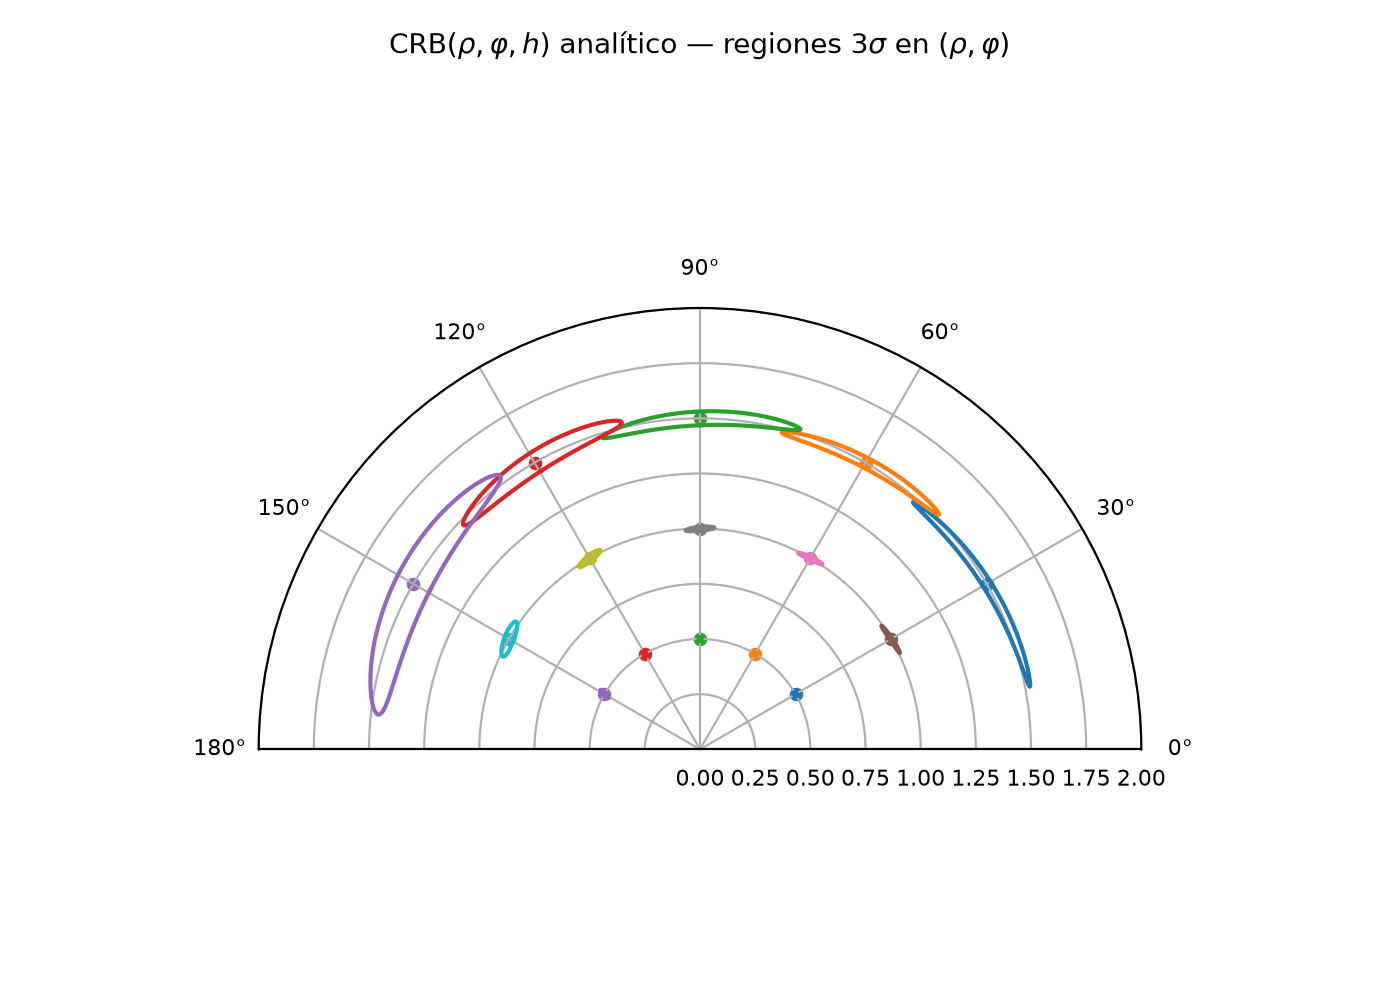
\includegraphics[width=0.86\textwidth]{../plots/crb_standard_regions_analytic.png}
\caption{CRB$(\rho,\varphi,h)$ \emph{anal\'itico} (dos rebotes, cuatro cosenos,
$4\pi^2$): regiones $3\sigma$ en $(\rho,\varphi)$, generadas con derivadas
cerradas. Archivo \texttt{plots/crb\_standard\_regions\_analytic.png}.}
\label{fig:analytic-regions}
\end{figure}

\subsection{Superposici\'on anal\'itico vs FD}
Comparamos contra el m\'etodo rasterizado / diferencias finitas, cuyo grid se
carga de \texttt{plots/crb\_grid\_results.pkl} (generado por
\texttt{regenerate\_crb\_standard\_regions.py}).

\begin{remark}[Las figuras de comparaci\'on corresponden a la corrida FD previa]
No re-ejecutamos el rasterizador (cuesta horas). Las superposiciones usan el
grid FD ya disponible en la cache (\emph{fixed\_h}, dos par\'ametros
$[\rho,\varphi]$, comparaci\'on \emph{apples-to-apples}). Esa corrida FD emple\'o
\emph{exactamente} los valores del simulador que ahora tambi\'en usa el anal\'itico
(\texttt{camera\_FOV}$=0.25$, $64\times64$, \texttt{bin\_size}$=3.9\times10^{-10}$,
\texttt{laser\_intensity}$=1000$, \texttt{background}$=0.1$, $w=0.5$, $h=1$), de
modo que la comparaci\'on de \textbf{magnitud} (y de forma) es leg\'itima: ambas
rutas comparten normalizaci\'on y rejilla.
\end{remark}

\begin{remark}[Misma escala f\'isica, pero sesgo de cuadratura sistem\'atico]
Con la amplitud f\'isica ($I_{\mathrm{laser}}=1000$, \'area $A_{\mathrm{eff}}=w h$,
Obs.~\ref{rem:area}) y la misma rejilla $64\times64$/\texttt{bin} real del
simulador, el CRB anal\'itico y el FD quedan en las \textbf{mismas unidades} / la
misma escala f\'isica --- esto corrige el defecto de la versi\'on previa (ganancia
$G$ y rejilla $8\times8$ arbitrarias). \textbf{Pero no coinciden en tama\~no}:
sobre el grid \emph{fixed\_h} el anal\'itico da $\sim0.5$--$0.7\times$ la $\sigma$
del FD (p.\,ej.\ en $(1,90^\circ)$:
$\sigma_\rho^{\mathrm{an}}=2.3\times10^{-3}$ vs
$\sigma_\rho^{\mathrm{FD}}=4.2\times10^{-3}$\,m;
$\sigma_\varphi^{\mathrm{an}}=1.1^\circ$ vs $\sigma_\varphi^{\mathrm{FD}}=1.4^\circ$;
la raz\'on $\sigma_\varphi^{\mathrm{an}}/\sigma_\varphi^{\mathrm{FD}}$ baja hasta
$\sim0.57$). Ese desfase es el \textbf{sesgo de cuadratura puntual}
(Obs.~\ref{rem:cuadratura}): la faceta puntual sobreestima la intensidad
$\sim1.5\times$ (dominado por oclusi\'on) y por tanto \emph{subestima} el CRB.
\textbf{No} se cierra endureciendo el suavizado --- eso lleva al forward duro
\emph{puntual}, no al de malla --- sino sumando sobre malla (rama (a)+(b)+(c)).
La superposici\'on \emph{normalizada en forma} (Fig.~\ref{fig:avf-shape}) sirve
para comparar orientaci\'on/aspecto sin el factor de tama\~no.
\end{remark}

\begin{figure}[ht]
\centering
\IfFileExists{../plots/crb_regions_analytic_vs_fd.png}{%
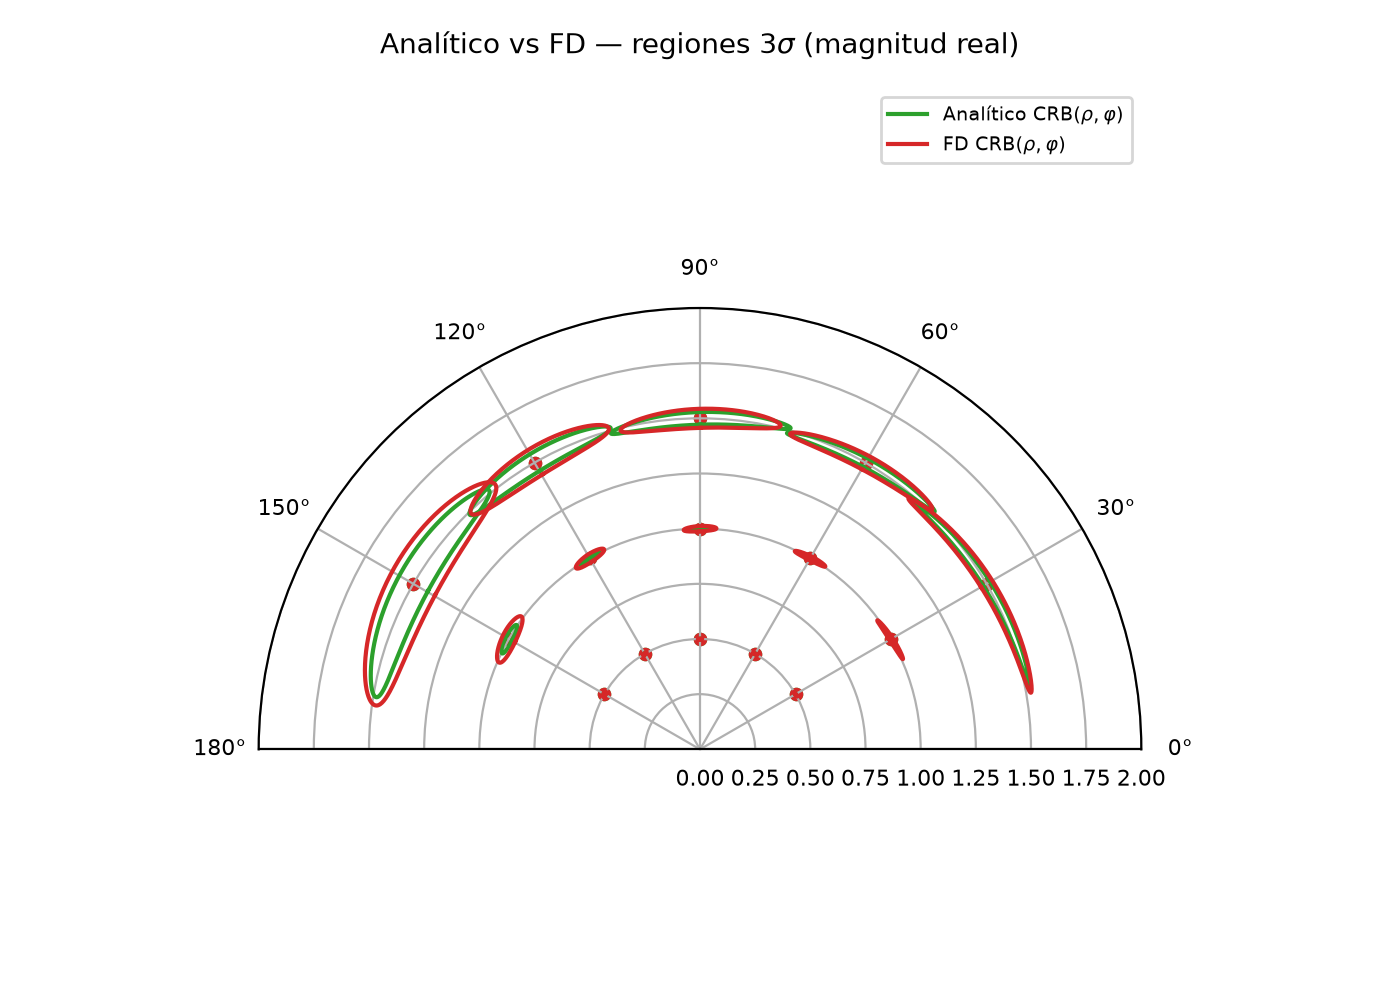
\includegraphics[width=0.72\textwidth]{../plots/crb_regions_analytic_vs_fd.png}%
}{\textit{(Pendiente: ejecutar la comparaci\'on con la cache FD disponible.)}}
\caption{(a) Superposici\'on anal\'itico (verde, dos rebotes, amplitud f\'isica
$I_{\mathrm{laser}}\!\cdot\!w h$, rejilla $64\times64$) vs FD (rojo) a
\emph{magnitud real}: con la variante (a)+(b) ambas elipses $3\sigma$ viven en la
\textbf{misma escala f\'isica} y su orientaci\'on concuerda, pero la anal\'itica es
sistem\'aticamente \textbf{m\'as peque\~na} ($\sim0.5$--$0.7\times$) por el sesgo de
cuadratura puntual (Obs.~\ref{rem:cuadratura}); \textbf{no} coinciden en tama\~no ni
lo har\'an al endurecer el suavizado. Archivo
\texttt{plots/crb\_regions\_analytic\_vs\_fd.png}.}
\label{fig:avf-abs}
\end{figure}

\begin{figure}[ht]
\centering
\IfFileExists{../plots/crb_regions_analytic_vs_fd_shapenorm.png}{%
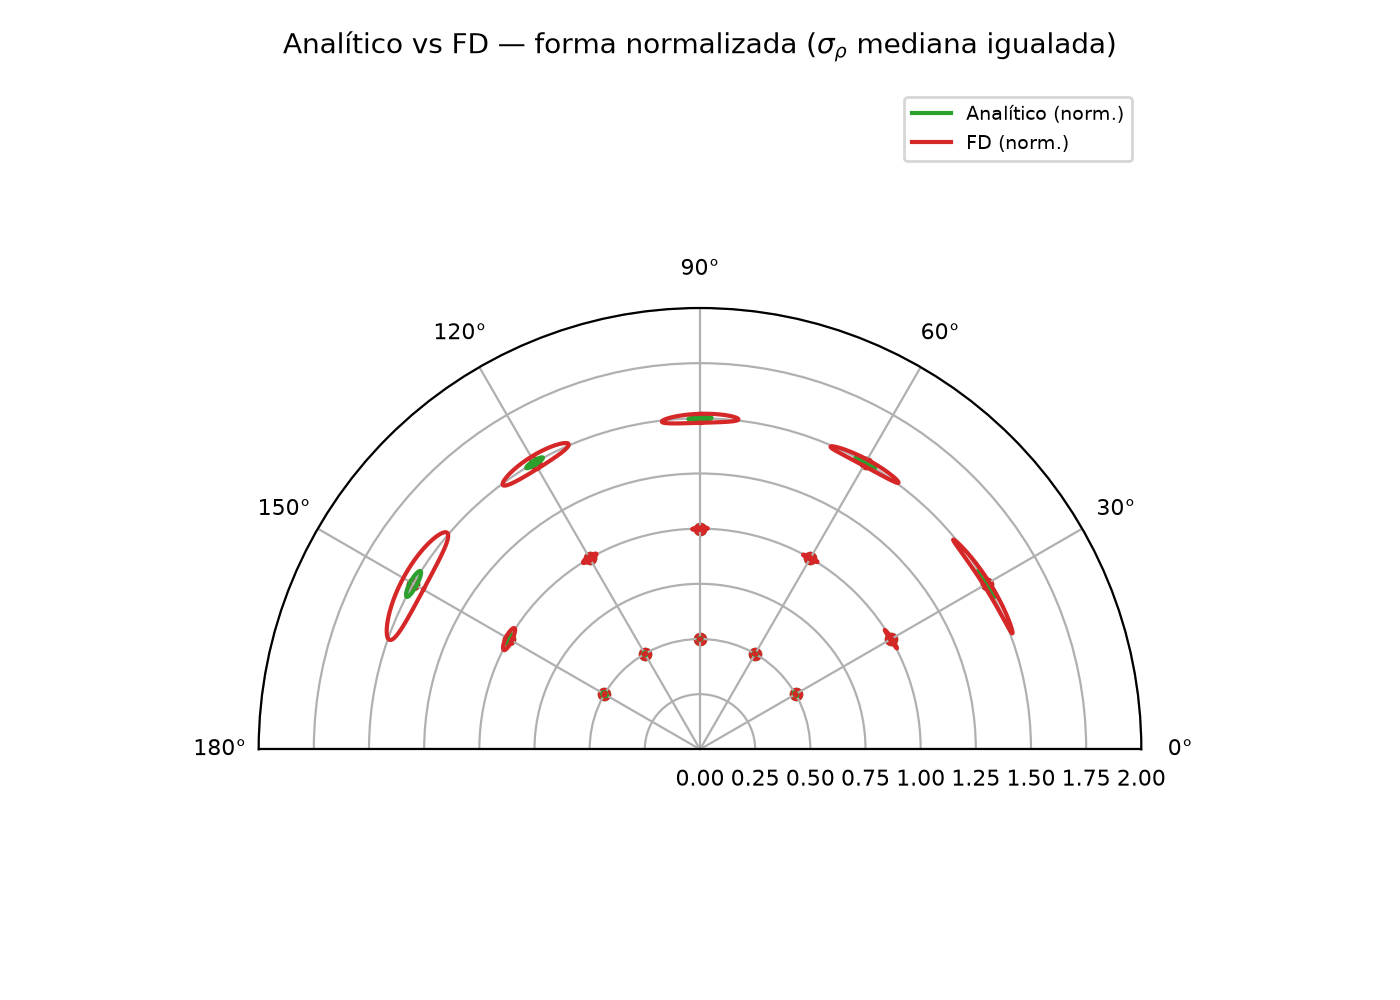
\includegraphics[width=0.72\textwidth]{../plots/crb_regions_analytic_vs_fd_shapenorm.png}%
}{\textit{(Pendiente: ejecutar la comparaci\'on con la cache FD disponible.)}}
\caption{(b) Superposici\'on \emph{normalizada en forma} ($\sigma_\rho$ mediana
igualada): compara orientaci\'on y aspecto, no el tama\~no.
Archivo \texttt{plots/crb\_regions\_analytic\_vs\_fd\_shapenorm.png}.}
\label{fig:avf-shape}
\end{figure}

\subsection{Tabla num\'erica resumida}
La Tabla~\ref{tab:avf} resume las desviaciones y la \textbf{relaci\'on de
aspecto} (eje mayor/menor de la elipse $3\sigma$) de cada m\'etodo; la tabla
completa (con la inclinaci\'on \emph{tilt}) est\'a en
\texttt{docs/analytic\_vs\_fd\_comparison.txt}.

\IfFileExists{analytic_vs_fd_table.tex}{% Auto-generated by generate_analytic_crb_plots.py -- do not edit by hand.
\begin{table}[ht]
\centering\small
\caption{CRB anal\'itico vs FD sobre el grid $[\rho,\varphi]$ (\emph{fixed\_h}). $\sigma_\rho$ en m, $\sigma_\varphi$ en grados; \emph{asp}$=$eje mayor/menor de la elipse $3\sigma$ en $(\rho,\varphi)$. Magnitudes absolutas no comparables (modelos distintos); comparar \emph{asp} y la forma.}
\label{tab:avf}
\begin{tabular}{@{}rr|rrr|rrr@{}}
\toprule
 & & \multicolumn{3}{c|}{Anal\'itico} & \multicolumn{3}{c}{FD (rasterizado)} \\
$\rho$ & $\varphi^\circ$ & $\sigma_\rho$ & $\sigma_\varphi$ & asp & $\sigma_\rho$ & $\sigma_\varphi$ & asp \\
\midrule
0.5 & 30 & 0.005255 & 1.73 & 7.0 & 0.0006859 & 0.509 & 19.2 \\
0.5 & 60 & 0.004762 & 1.16 & 4.5 & 0.0006779 & 0.44 & 14.0 \\
0.5 & 90 & 0.005615 & 1.16 & 3.7 & 0.0007805 & 0.385 & 9.6 \\
0.5 & 120 & 0.008278 & 1.01 & 2.2 & 0.001116 & 0.412 & 7.1 \\
0.5 & 150 & 0.01454 & 1.46 & 1.8 & 0.001847 & 0.548 & 5.7 \\
1.0 & 30 & 0.005748 & 2.26 & 10.1 & 0.003406 & 2.01 & 13.1 \\
1.0 & 60 & 0.004987 & 1.57 & 6.3 & 0.003448 & 1.48 & 8.2 \\
1.0 & 90 & 0.00585 & 1.64 & 5.2 & 0.004197 & 1.42 & 6.2 \\
1.0 & 120 & 0.008383 & 1.42 & 3.0 & 0.006299 & 1.46 & 4.2 \\
1.0 & 150 & 0.01434 & 2.08 & 2.6 & 0.01086 & 2.21 & 3.7 \\
1.5 & 30 & 0.0102 & 4.11 & 11.2 & 0.01207 & 6.76 & 12.1 \\
1.5 & 60 & 0.00874 & 2.98 & 7.0 & 0.01215 & 4.69 & 7.2 \\
1.5 & 90 & 0.01025 & 3.31 & 6.1 & 0.01486 & 4.66 & 5.7 \\
1.5 & 120 & 0.01454 & 2.83 & 3.5 & 0.02185 & 4.72 & 3.8 \\
1.5 & 150 & 0.02478 & 4.28 & 3.0 & 0.03747 & 7.43 & 3.5 \\
\bottomrule
\end{tabular}
\end{table}
}{%
\textit{(Tabla pendiente: ejecutar \texttt{generate\_analytic\_crb\_plots.py}
con la cache FD disponible.)}}

\subsection{\textup{?`}Cu\'al elipse es ``mejor''?}
Ahora que las escalas comparten unidades, ``mejor'' combina \textbf{escala
f\'isica correcta}, \textbf{calidad/suavidad de la derivada} y \textbf{sensatez de
la forma} --- teniendo presente el sesgo de cuadratura:
\begin{enumerate}[nosep]
    \item \textbf{Escala (no magnitud exacta).} Con la variante (a)+(b) el CRB
    anal\'itico y el FD est\'an en las \textbf{mismas unidades} (normalizaci\'on
    $I_{\mathrm{laser}}\!\cdot\!w h$, misma rejilla). Pero el anal\'itico es
    sistem\'aticamente \textbf{menor} ($\sim0.5$--$0.7\times$ la $\sigma$ del FD)
    por el \textbf{sesgo de cuadratura puntual} (Obs.~\ref{rem:cuadratura}); ese
    desfase \textbf{no} se cierra al endurecer el suavizado (que lleva al forward
    duro \emph{puntual}, no al de malla), sino con la suma sobre malla (a+b+c).
    \item \textbf{Suavidad / condicionamiento.} El forward anal\'itico tiene
    derivadas \emph{exactas} ($C^\infty$). El Jacobiano FD se calcula sobre un
    forward con escalones ($\lceil\cdot\rceil$ y $\texttt{xint}>0$ constantes a
    trozos), mezclando mesetas planas y saltos de bin (ruido de discretizaci\'on,
    dependencia de $\delta$). La elipse anal\'itica es la \textbf{mejor
    condicionada}.
    \item \textbf{Forma / orientaci\'on.} Ambos dan elipses finas en \'angulo
    (resoluci\'on azimutal de la arista) y m\'as anchas en rango; la orientaci\'on
    es consistente. El aspecto medio difiere ($9.36$ anal.\ vs $8.22$ FD), en
    parte por el sesgo puntual y en parte porque los anchos de suavizado
    ($\kappa=60$, $\tau=\Delta t$) son \textbf{gen\'ericos y m\'as gruesos} que la
    discretizaci\'on (penumbra $\sim4.3$ p\'ixeles); la rama (a)+(b)+(c) los ata a
    la discretizaci\'on ($\kappa=256$, $\tau=\Delta t/\sqrt{12}$).
    \item \textbf{Salvedad.} La faceta puntual (\'area \'unica $w h$ en $z=h/2$)
    \textbf{no} reproduce el rasterizador de malla; el sesgo es \emph{sistem\'atico}
    (no un residual que se anule) y solo lo corrige la suma sobre malla.
\end{enumerate}
\textbf{Veredicto:} (a)+(b) coloca el CRB anal\'itico en la \textbf{escala f\'isica
correcta} (mismas unidades que la FD) y, por sus derivadas exactas, mejor
condicionada; pero conserva un sesgo de cuadratura puntual sistem\'atico que hace
el CRB \emph{menor} que el de malla. El FD sigue siendo la referencia (modelo de
malla completo); la correcci\'on del sesgo es la rama (a)+(b)+(c).

%==============================================================================
\section{Conclusi\'on}
\label{sec:conclusion}
%==============================================================================

Partimos de la \textbf{funci\'on que usa el simulador} (celda~8: dos rebotes,
cuatro cosenos, $4\pi^2$, \texttt{ceil}, \texttt{xint}$>0$) --- no del modelo del
\emph{writeup} --- y la volvimos $C^\infty$ reemplazando sus tres
discontinuidades por an\'alogos cerrados, justificando \emph{por qu\'e} cada
elecci\'on: la masa de Dirac en un bin por la \textbf{integral gaussiana}
\eqref{eq:erf-bin} (diferencia de $\erf$, el coraz\'on de la
diferenciabilidad), el Heaviside de la \texttt{xint} por una \textbf{sigmoide}
\eqref{eq:sigmoid}, y los cuatro $\max(0,\cdot)$ por \textbf{softplus}
\eqref{eq:softplus}. Con ello:
\begin{itemize}[nosep]
    \item las derivadas $\partial g/\partial\rho,\partial g/\partial\varphi,
          \partial g/\partial h$ son \textbf{exactas} (\texttt{sympy}), sin
          ajustar el paso $\delta$;
    \item $g_q$ y sus derivadas est\'an \textbf{bien definidas en $0$} por el
          fondo $b>0$ (sin piso $\varepsilon$);
    \item la Fisher y el CRB \eqref{eq:fisher}--\eqref{eq:crb} conservan la
          estructura Poisson;
    \item la validaci\'on anal\'itico-vs-FD da error m\'aximo relativo
          $\sim1\times10^{-9}$;
    \item con \textbf{amplitud f\'isica} ($I_{\mathrm{laser}}\!\cdot\!w h$) y la
          \textbf{misma rejilla} $64\times64$/\texttt{bin} real (variante
          (a)+(b)), el CRB anal\'itico y el FD quedan en las \textbf{mismas
          unidades} / la misma escala f\'isica (se corrige el defecto de escala de
          la versi\'on previa con ganancia y rejilla propias).
\end{itemize}
\textbf{Salvedad principal (sesgo de cuadratura, no convergencia).} La variante
(a)+(b) corrige la \emph{escala} pero \textbf{no} la magnitud: es una faceta
\textbf{puntual}, i.e.\ una \textbf{cuadratura de un solo nodo} (\'area $w h$ en el
centroide $z=h/2$) de la integral que el simulador suma sobre malla. Su error es
\textbf{sistem\'atico} --- sobreestima la intensidad $\sim1.5\times$ (dominado por
la oclusi\'on de la faceta extendida; adem\'as $1/d_2^2$ y cosenos no lineales) ---
y por eso el CRB anal\'itico es \emph{menor} que el FD ($\sigma_\varphi$ anal./FD
hasta $\sim0.57$). Endurecer el suavizado \textbf{no} lo corrige: en el l\'imite
$\tau\to0,\kappa,\beta\to\infty$ esta variante converge a su \textbf{propio}
forward duro \emph{puntual} (verificado: $L^1$ $15.9\%\to0.34\%$), \textbf{no} al
de malla (Obs.~\ref{rem:cuadratura}). La correcci\'on es la \textbf{suma sobre
malla} (rama (a)+(b)+(c)), que adem\'as ata los anchos de suavizado a la
discretizaci\'on ($\kappa=256=1/$p\'ixel, $\tau=\Delta t/\sqrt{12}$) en lugar de
los gen\'ericos de aqu\'i ($\kappa=60$, penumbra $\sim4.3$ p\'ixeles;
$\tau=\Delta t$). Otras salvedades: la geometr\'ia (rejilla del simulador) es fija;
se asume $\nabla d_i\neq\vect0$ (Hip.~\ref{as:geom}) e $\matr{I}\succ0$.

%------------------------------------------------------------------------------
\paragraph{Archivos.}
\texttt{crb\_analytic\_forward.py} (forward de dos rebotes $+$ Jacobiano
simb\'olico $+$ CRB), \texttt{validate\_analytic\_forward.py} (validaci\'on
anal\'itico vs FD), este documento \texttt{docs/analytic\_forward\_crb.tex}.
Reutiliza (sin modificar) \emph{helpers} de \texttt{crb\_polar\_functions.py}.

\end{document}
